\chapter{Secret appendix}
You are now reading the secret appendix!
A place hosting information classified due to reasons such as: high variance, unreliable controls, missing validations, partial knockouts, swapped labels, performed by undergrads, irregular proliferation, high background, bad antibodies, pipetting accidents, wrong volumes, low signal or just because it does not fit anywhere else.



\section{Integrated stress response}

\subsection{Aspartate depletion induced ISR}
Aspartate depletion is achieved in GOT DKO cells and shown to cause integrated stress response (ISR) both through eIF2a phosphorylation and ATF4 upregulation.
Media swapping induces a quick depletion of both Asp and Asn (figure \ref{fig:sapp:ISR:143B_GOT_DKO_ISR_conc}).
Asn efflux is likely more quick due to better permeability.
Upon Asn depletion the ISR cascade starts and can maintain high expression of ATF4 due to the continued Asn synthesis from Asp.
On the other hand, if Asp is depleted to the point of protein synthesis inhibition no signal might be detected when probing ATF4 as Asp levels will not recover.
We observe these dynamics clearly in HT1080 GOT DKO cells in figures \ref{fig:sapp:ISR:HT1080_DKO_ISR} and \ref{fig:sapp:ISR:HT1080_DKO_ASPtit_time}.
Especially, the ATF4 reporter shows the kinetics of these Asp/Asn depletion kinetics.

For 143B GOT DKO we observe similar results.
Here, inhibition of GCN2 ablates ATF4 expression while mitochondrial respiration (missing in rho0 cells) is not required for ATF4 upregulation.

\begin{figure}[t]
    \centering
    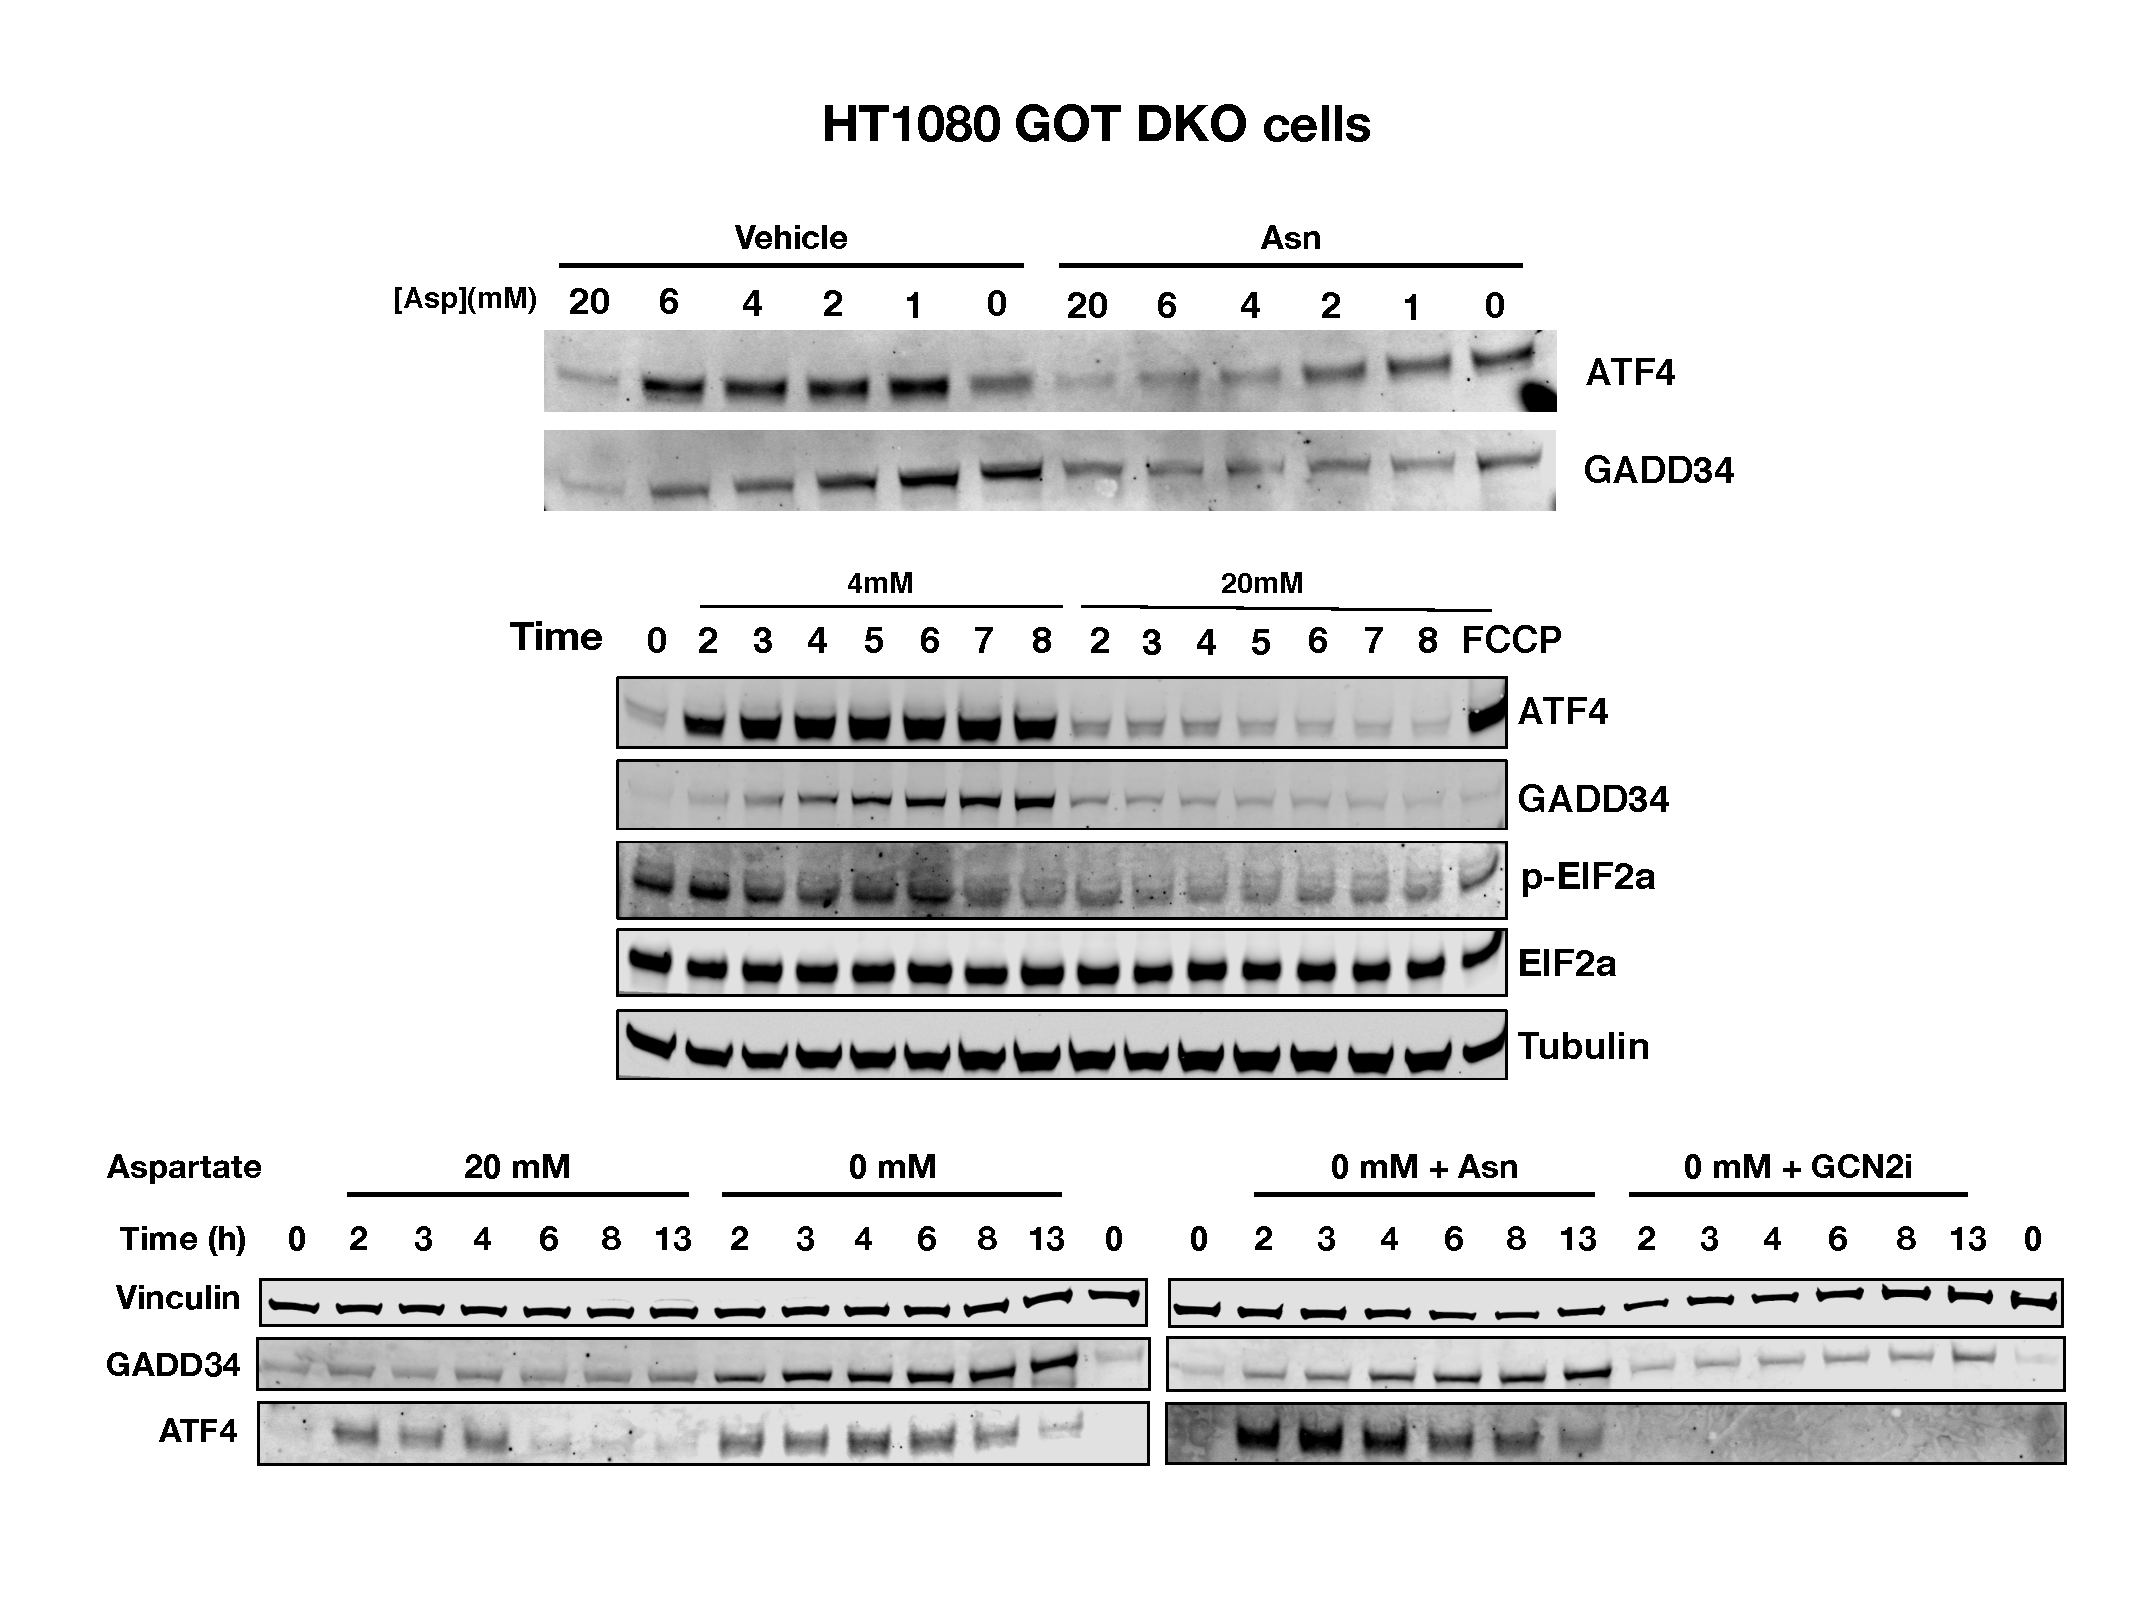
\includegraphics[width=0.99\textwidth]{figures/sapp/ISR/HT1080_DKO_ISR.pdf}
    \caption[Asp depl. induced ISR, HT1080 western]{
    Aspartate depletion in HT1080 GOT DKO cells initiated by media swapping.
    }
    \label{fig:sapp:ISR:HT1080_DKO_ISR}
\end{figure}

\begin{figure}[t]
    \centering
    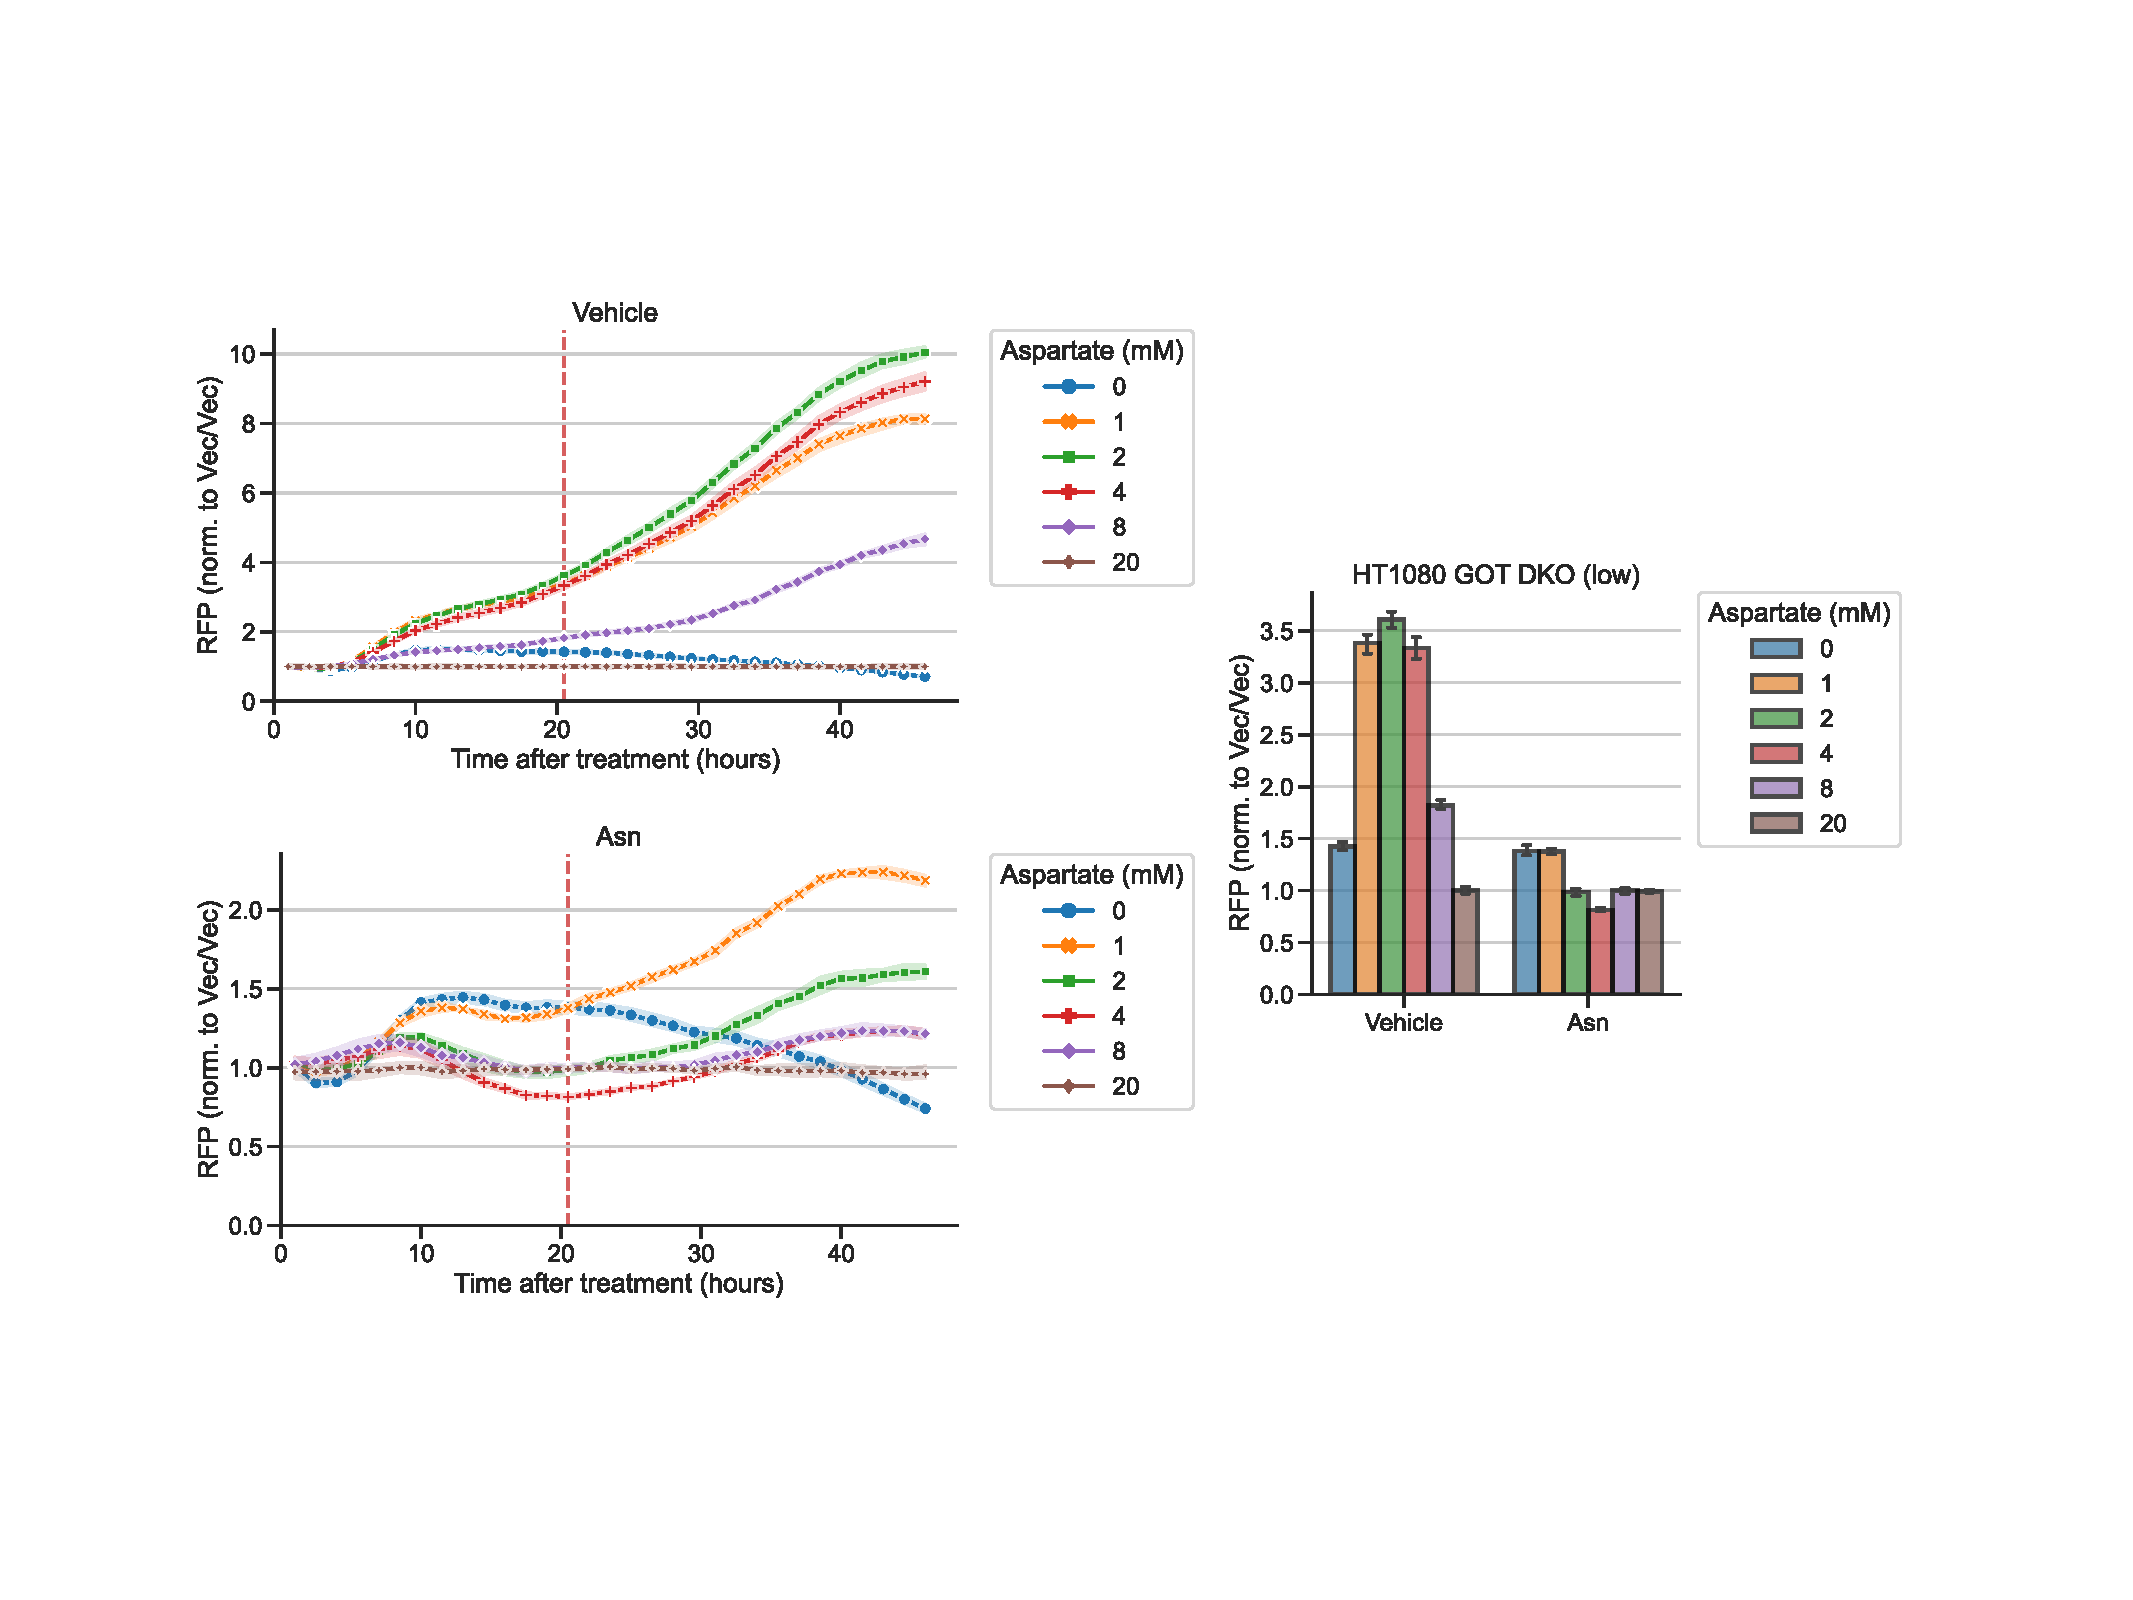
\includegraphics[width=0.98\textwidth]{figures/sapp/ISR/HT1080_DKO_ASPtit_time.pdf}
    \caption[Asp depl. induced ISR, HT1080 ATF4 reporter]{
    ATF4 reporter measurements after aspartate depletion in HT1080 GOT DKO (clone with low reporter at baseline).
    Vec/Vec normalization is normalization to the baseline condition (20 mM Asp, no Asn).
    Vertical red line on curve plot indicates time of measurements extracted for the barplot.
    }
    \label{fig:sapp:ISR:HT1080_DKO_ASPtit_time}
\end{figure}

\begin{figure}[t]
    \centering
    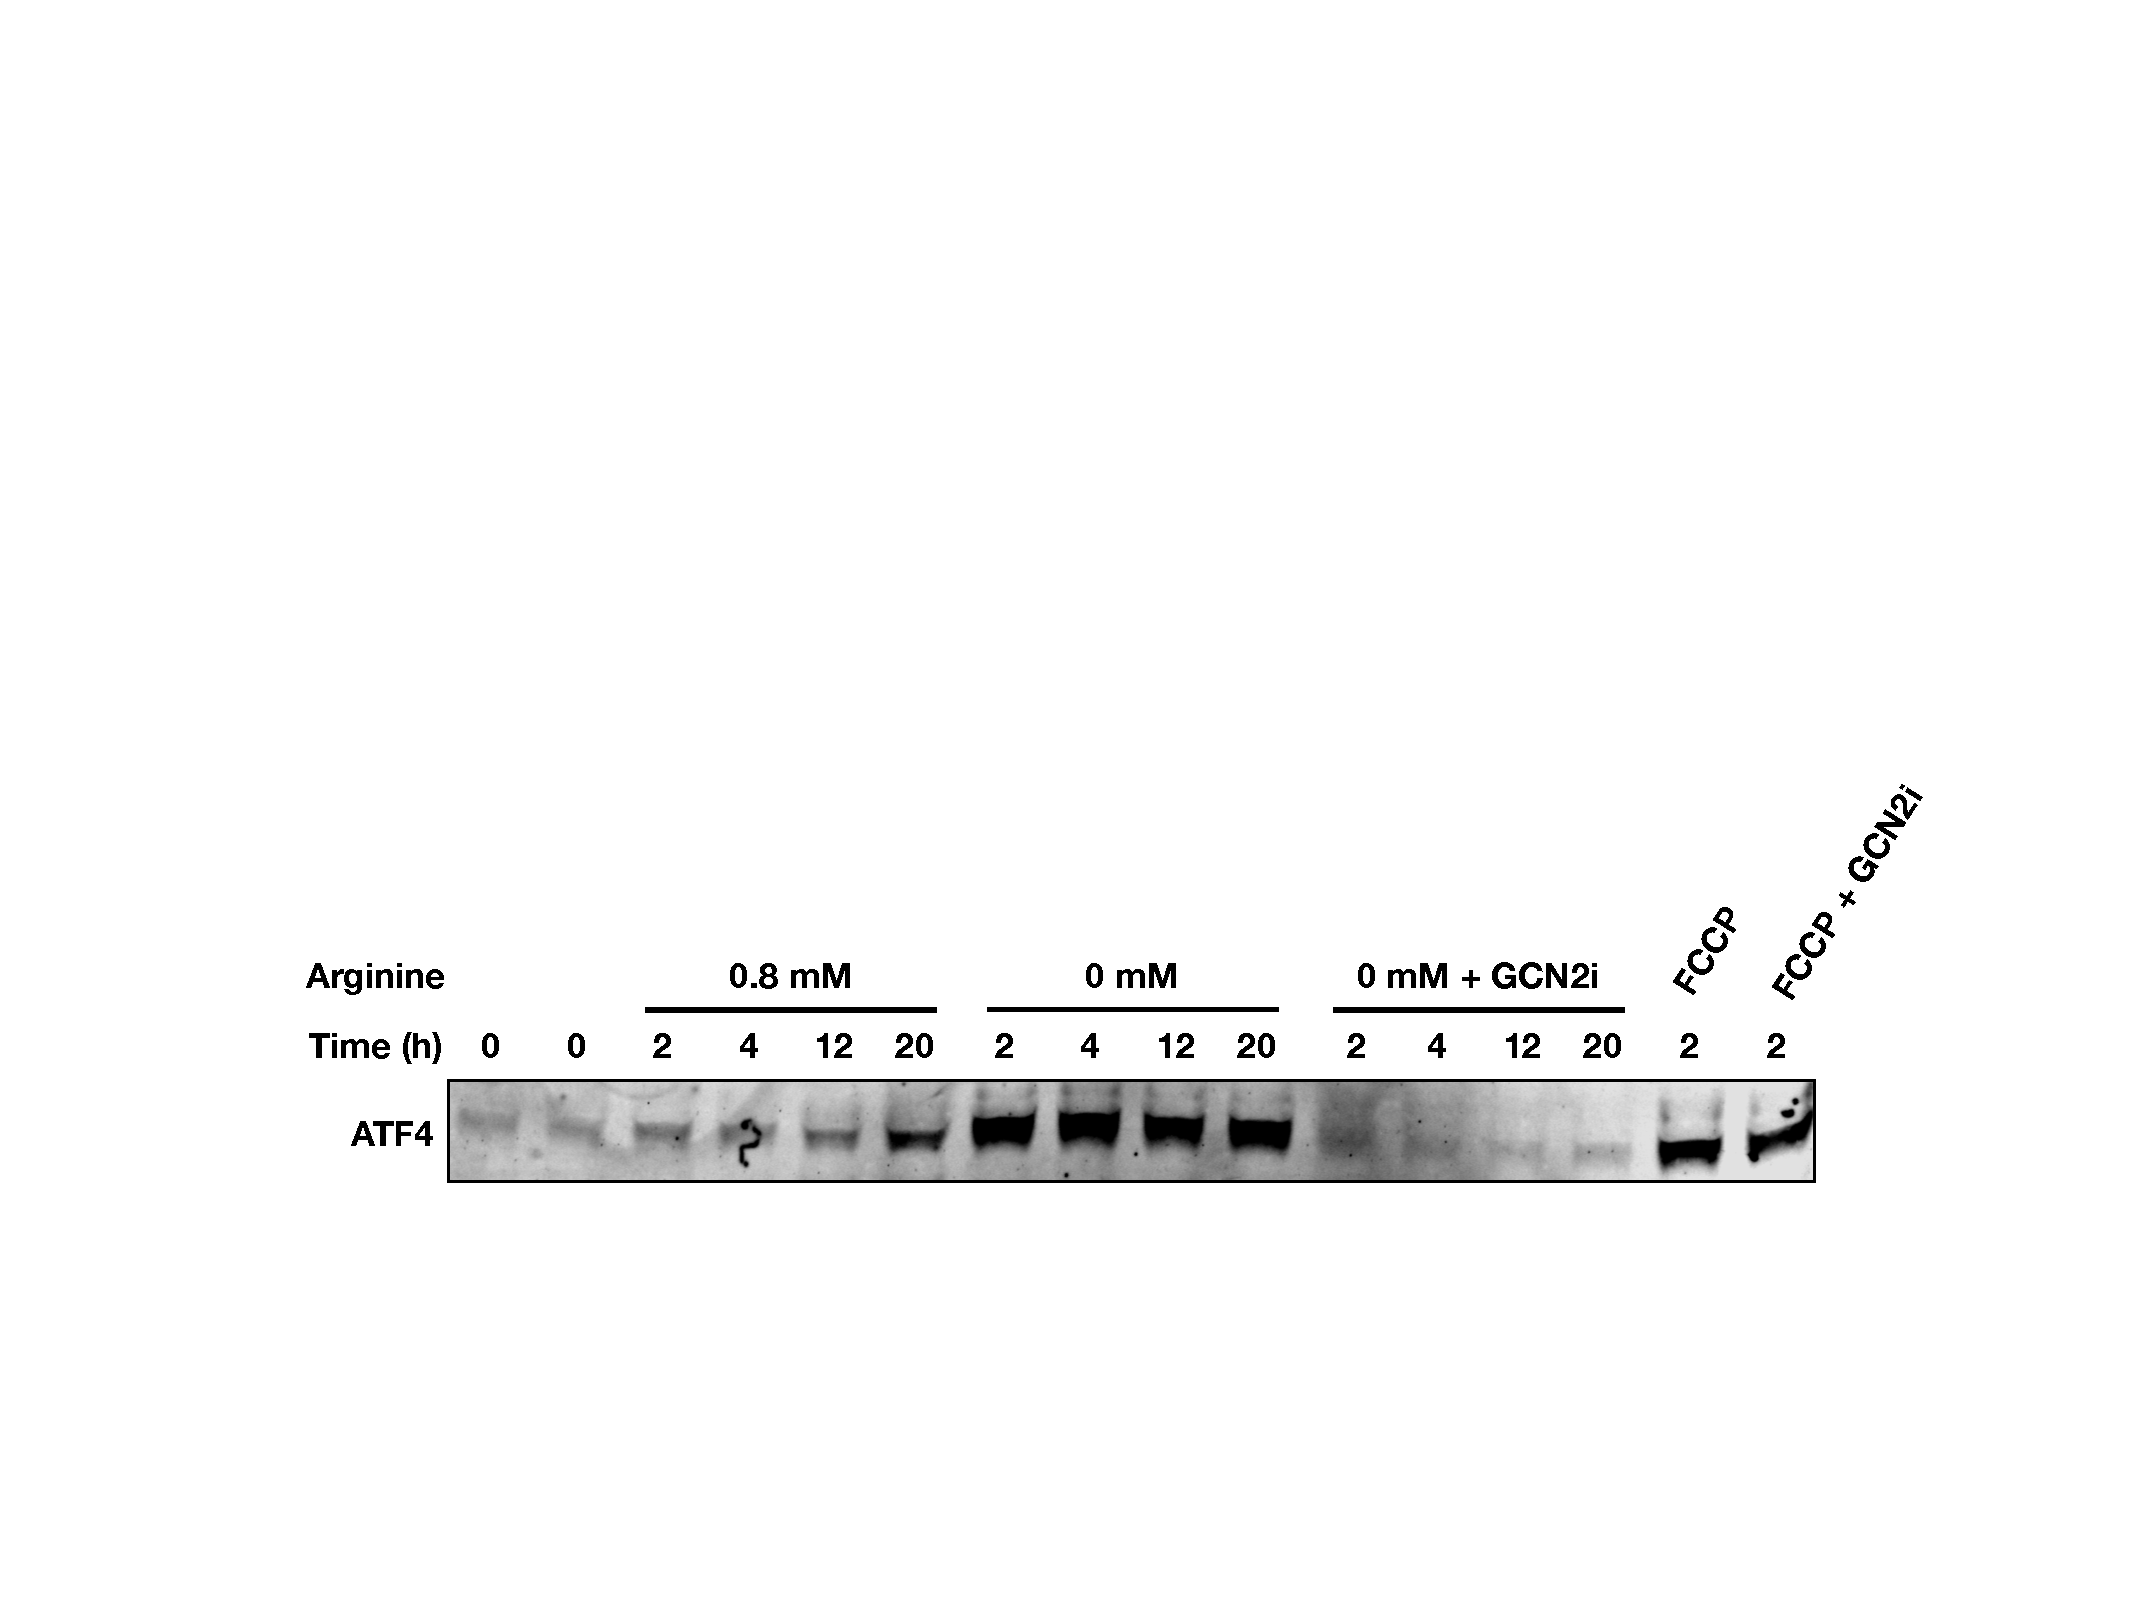
\includegraphics[width=0.60\textwidth]{figures/sapp/ISR/143B_GCN2i_val.pdf}
    \caption[GCN2 inhibitor validation]{
    Validation of activity and specificity of GCN2i in 143B WT cells.
    }
    \label{fig:sapp:ISR:143B_GCN2i_val}
\end{figure}

\begin{figure}[t]
    \centering
    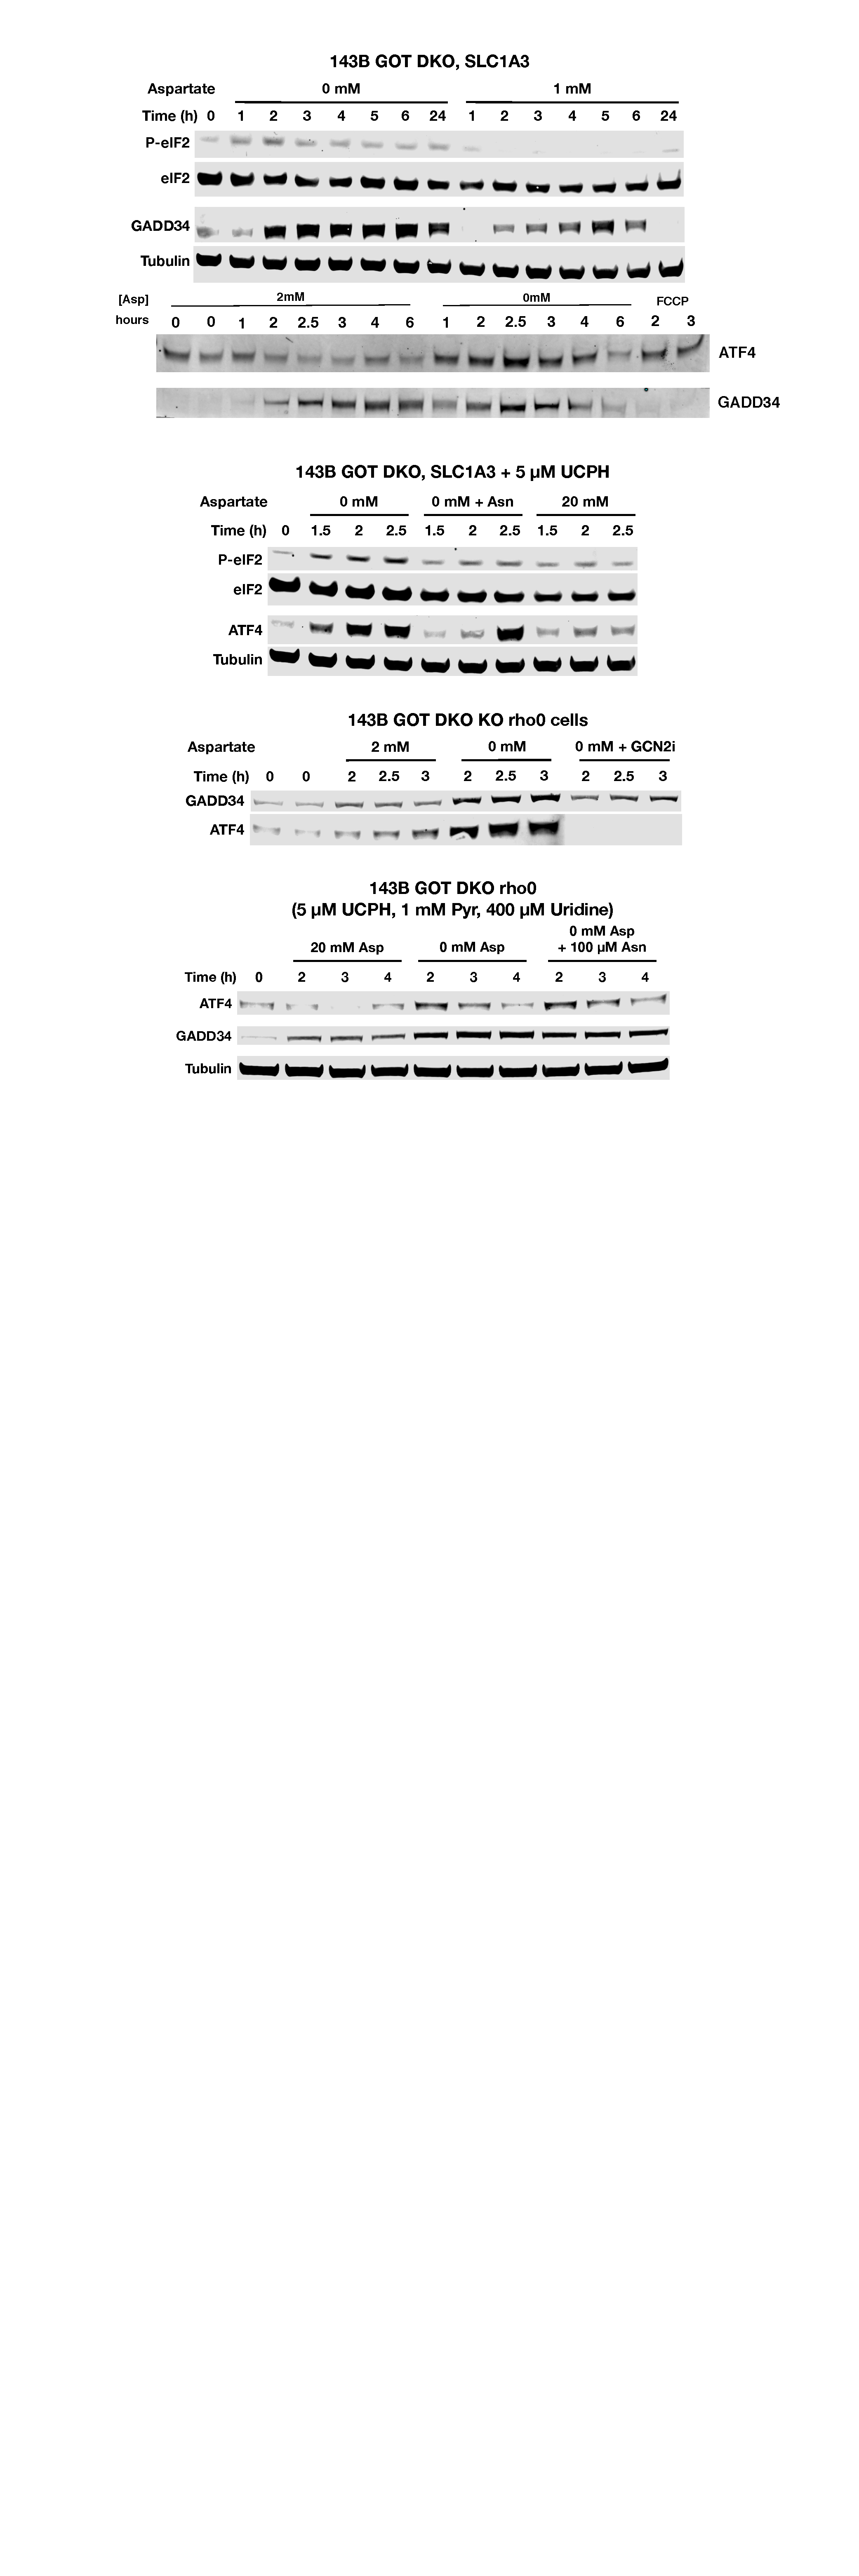
\includegraphics[height=0.85\textheight]{figures/sapp/ISR/143B_DKO_ISR.pdf}
    \caption[Asp depl. induced ISR, 143B western]{
    Aspartate depletion in 143B GOT DKO, SLC1A3 cells initiated by media swapping.
    }
    \label{fig:sapp:ISR:143B_DKO_ISR}
\end{figure}

\begin{figure}[!ht]
     \centering
     \begin{subfigure}[b]{0.35\textwidth}
         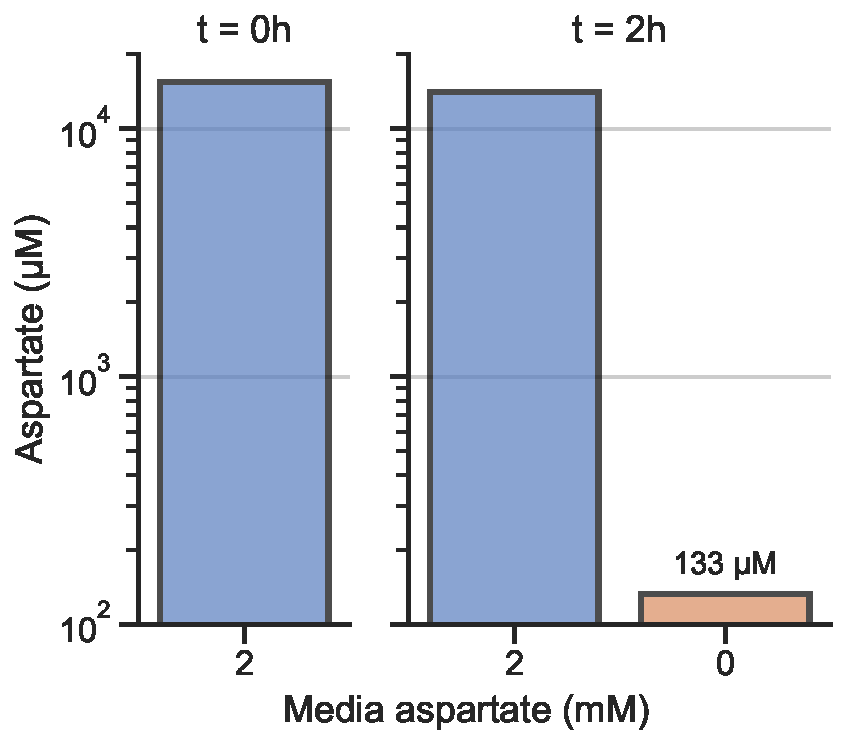
\includegraphics[width=\textwidth]{figures/sapp/ISR/143B_GOT_DKO_ISR_Asp_conc.pdf}
         \caption{Intracellular Asp}
         \label{fig:sapp:ISR:143B_GOT_DKO_ISR_Asp_conc}
     \end{subfigure}
     \hspace{0.02\textwidth}
     \begin{subfigure}[b]{0.35\textwidth}
         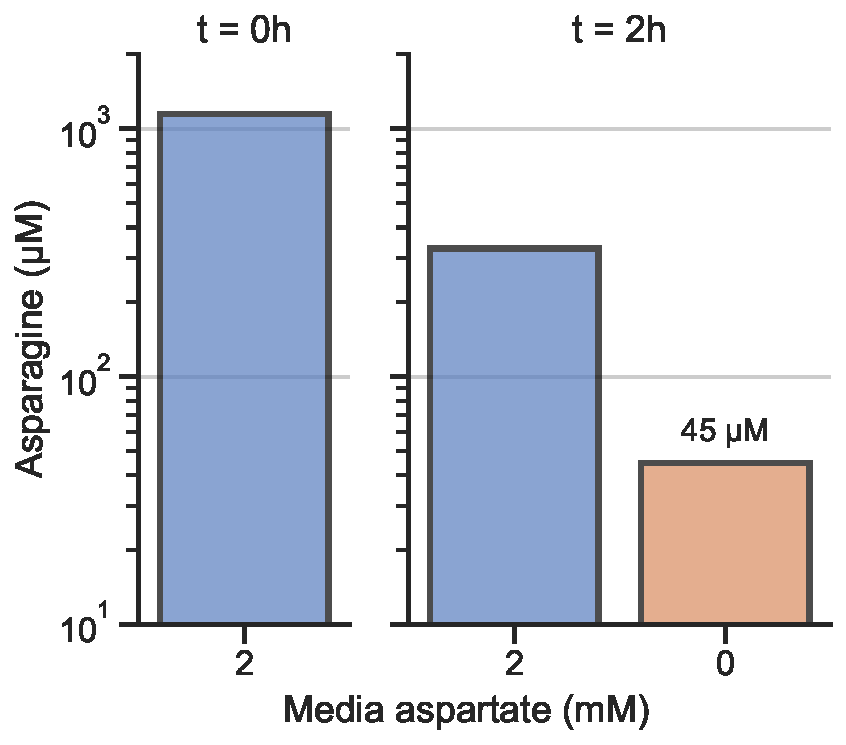
\includegraphics[width=\textwidth]{figures/sapp/ISR/143B_GOT_DKO_ISR_Asn_conc.pdf}
         \caption{Intracellular Asn}
         \label{fig:sapp:ISR:143B_GOT_DKO_ISR_Asn_conc}
     \end{subfigure}
     \hfill
        \caption[Intracellular Asp/Asn at ISR in GOT DKO]{
        Intracellular concentration of aspartate and asparagine before and 2 hours after media switch with/without aspartate for 143B GOT DKO cells, similar to figure \ref{fig:sapp:ISR:143B_DKO_ISR} (second panel from the top).
        }
        \label{fig:sapp:ISR:143B_GOT_DKO_ISR_conc}
\end{figure}





\FloatBarrier
\subsection{OMA1/HRI relation to rotenone/antimycin induced ISR}
According Fessler et al. and Guo et al. \cite{Fessler2020-zk, Guo2020-ia} OMA1/HRI is required for FCCP induced ISR.
Guo et al. also shows OMA1/HRI is required for rotenone/antimycin induced ISR (suppl. of Guo et al.).

We have pooled knockout cells (parental HT1080 ATF4 reporter low clone) of OMA1 and HRI.
These appear to ablate rotenone/antimycin induced ISR but strangely not FCCP induced ISR.
This could be due to pleiotropic effect of FCCP e.g. its is also depolarizing the plasma membrane and the lysosomal membrane.

\begin{figure}[!ht]
     \centering
     \begin{subfigure}[b]{0.49\textwidth}
         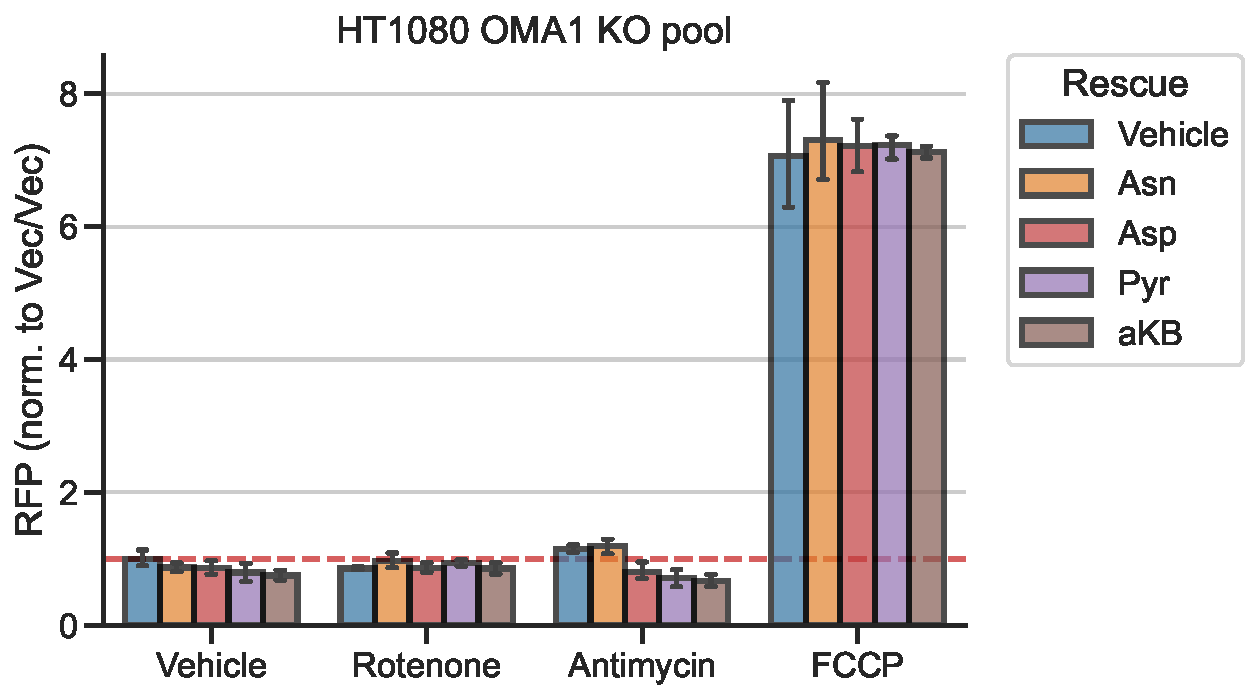
\includegraphics[width=\textwidth]{figures/sapp/ISR/ATF4rep_OMA1pool.pdf}
         \caption{OMA1 KO pool}
         \label{fig:sapp:ISR:ATF4rep_OMA1pool}
     \end{subfigure}
     \hfill
     \begin{subfigure}[b]{0.49\textwidth}
         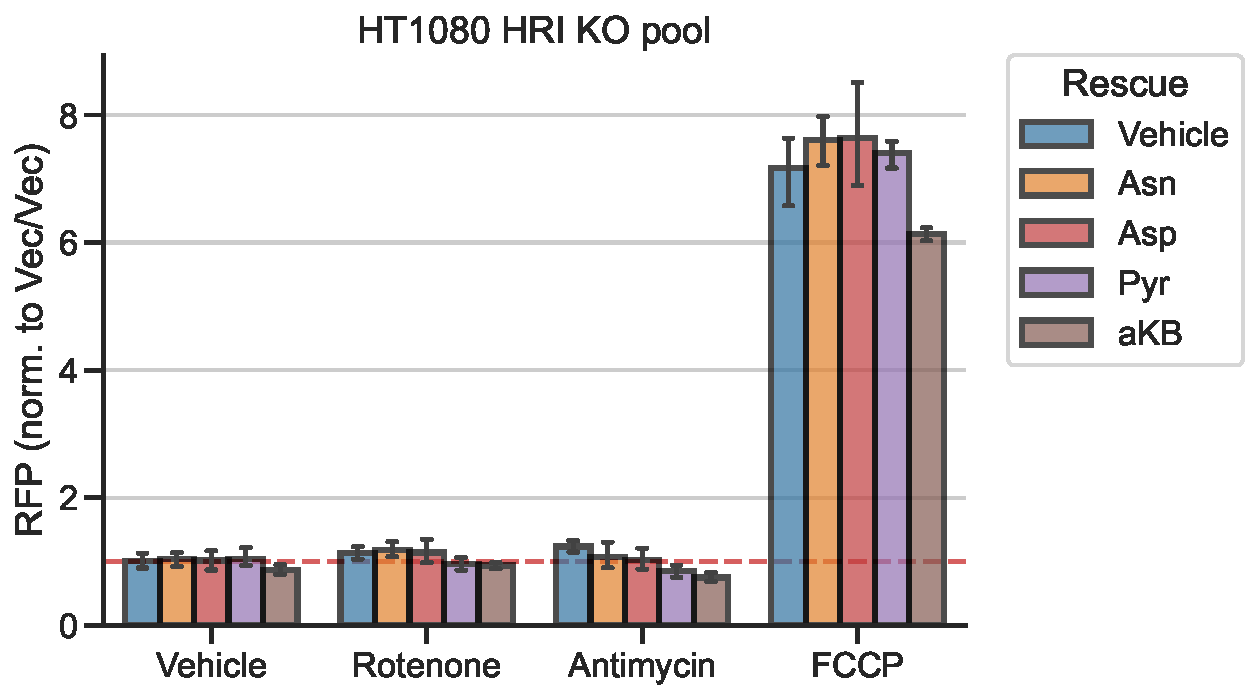
\includegraphics[width=\textwidth]{figures/sapp/ISR/ATF4rep_HRIpool.pdf}
         \caption{HRI KO pool}
         \label{fig:sapp:ISR:ATF4rep_HRIpool}
     \end{subfigure}
     \hfill
        \caption[ATF4 post mito inhib. OMA1/HRI KO, reporter]{
        ATF4 reporter assay measured 21 h after drug treatment with vehicle, rotenone (100 nM) or antimycin (1 µM) spiked-in as 10x.
        }
        \label{fig:sapp:ISR:ATF4rep_OMA1_HRIpool}
\end{figure}

\begin{figure}[t]
    \centering
    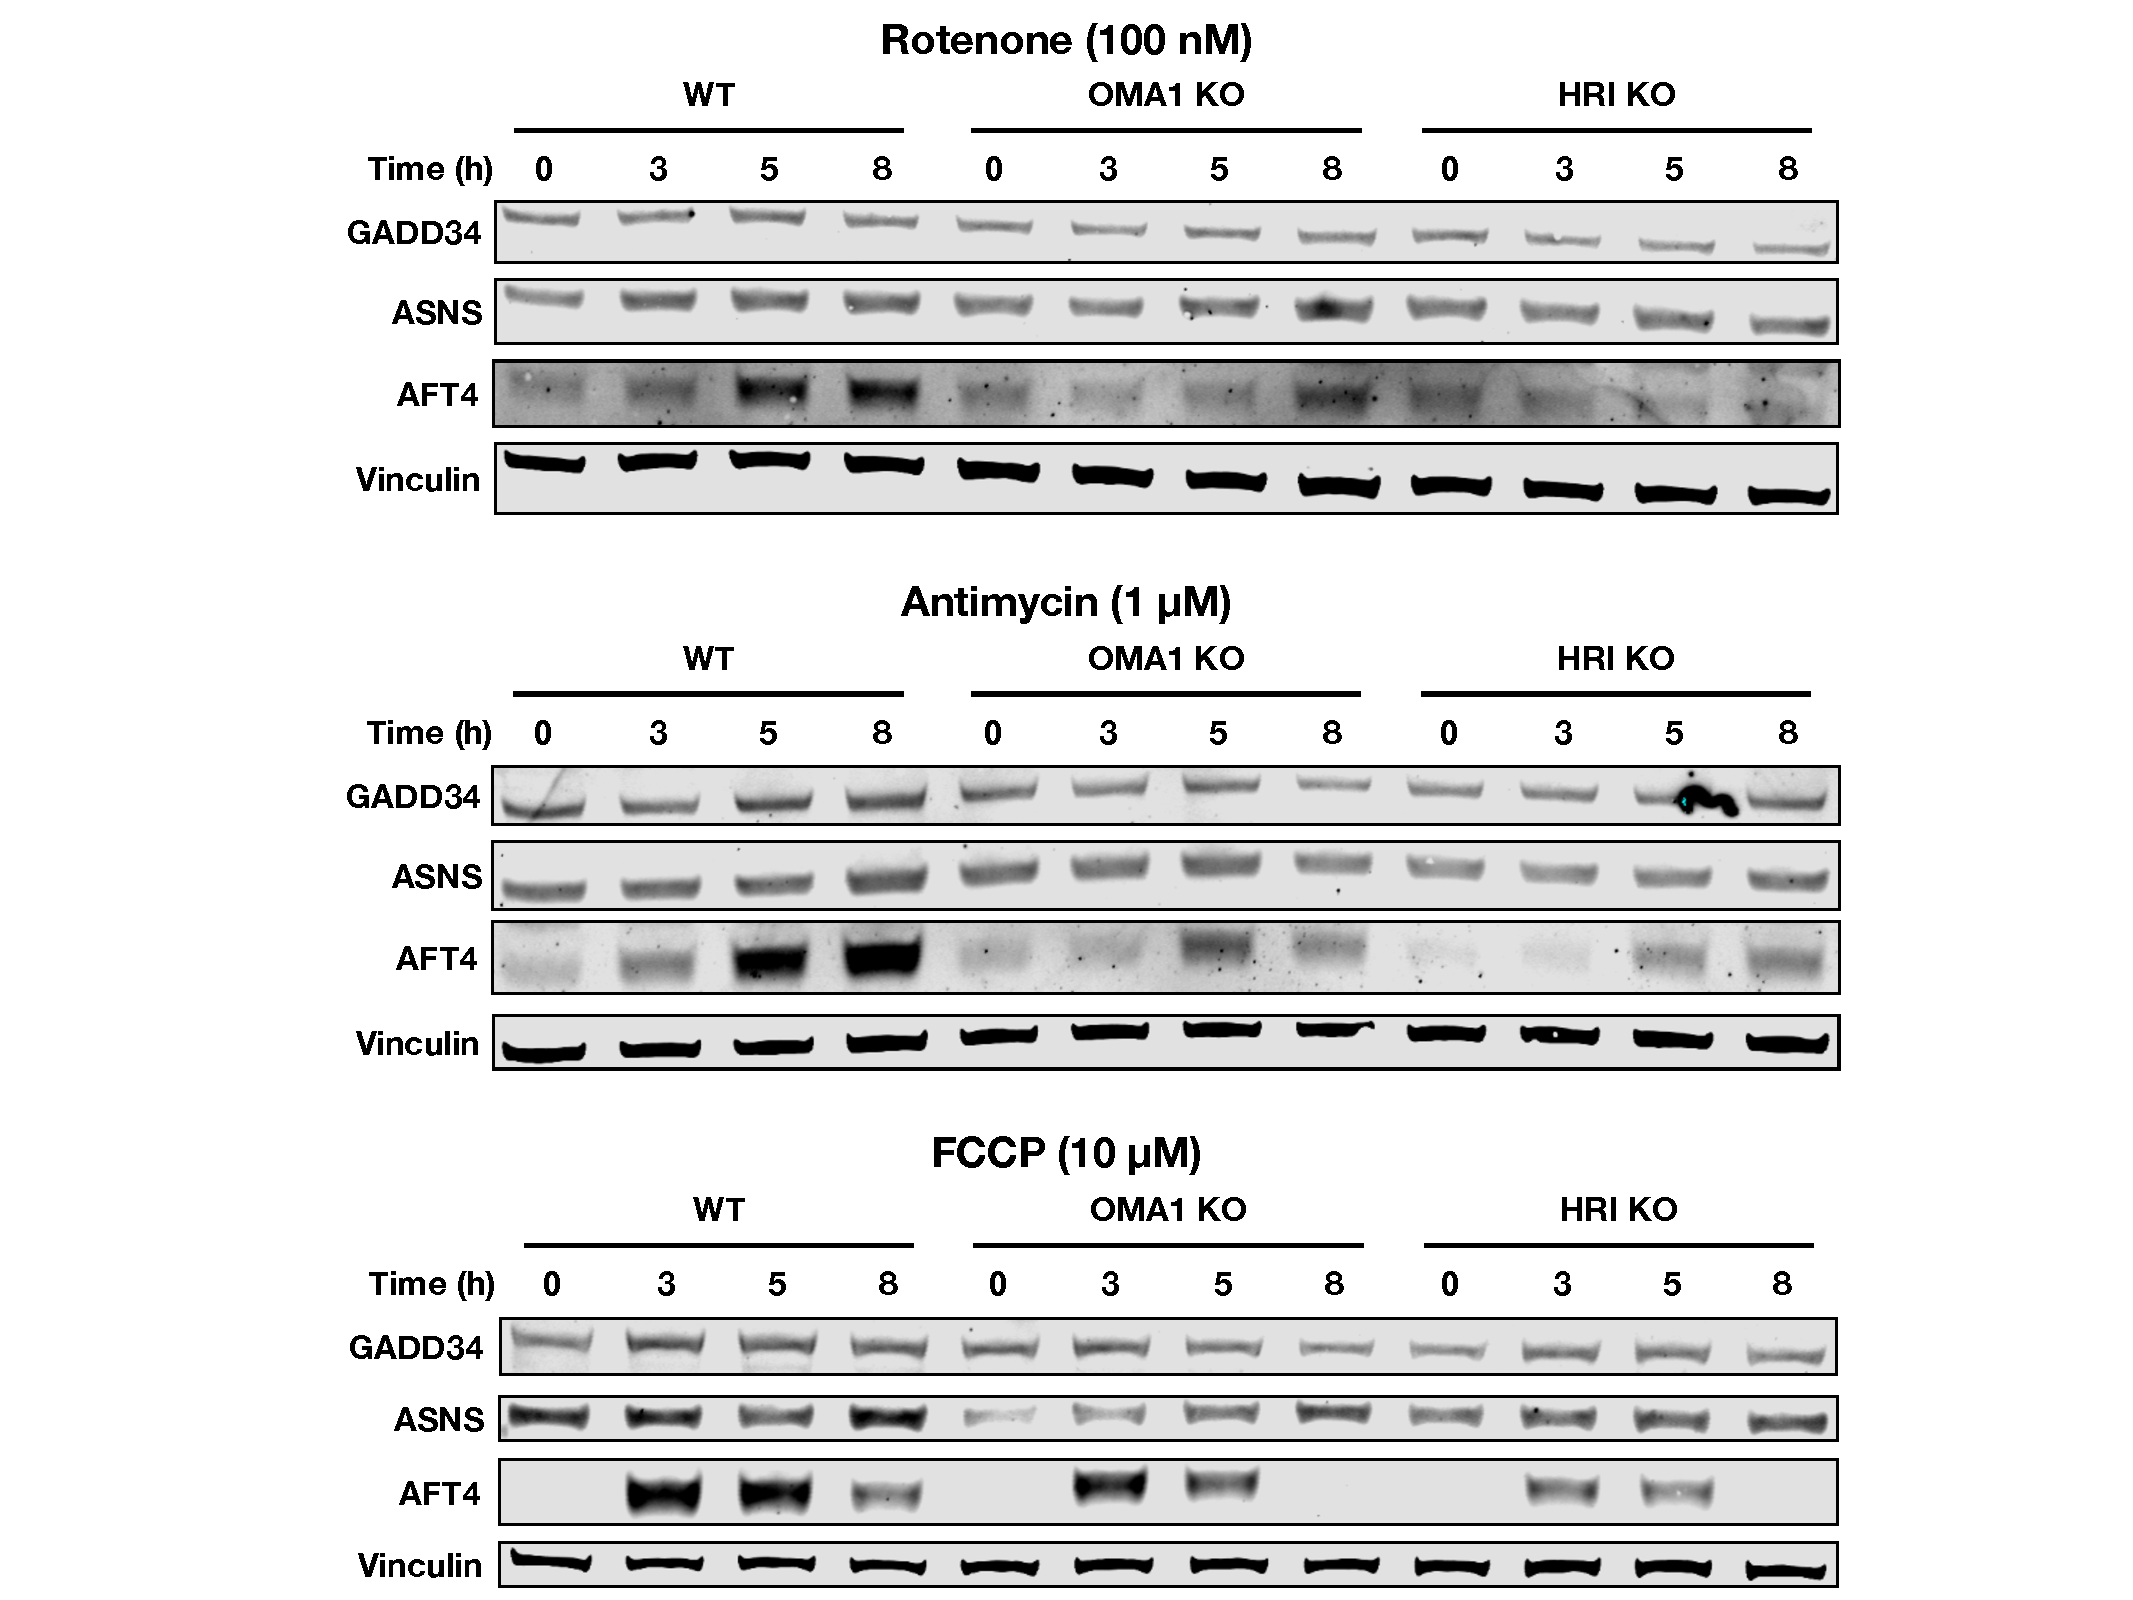
\includegraphics[width=0.65\textwidth]{figures/sapp/ISR/ATF4wes_OMA1_HRIpool.pdf}
    \caption[ATF4 post mito inhib. OMA1/HRI KO, western]{
    Same pooled knockout cells and handling as in figure \ref{fig:sapp:ISR:ATF4rep_OMA1_HRIpool}.
    Drugs spiked-in as 10x.
    }
    \label{fig:sapp:ISR:ATF4wes_OMA1_HRIpool}
\end{figure}






\FloatBarrier
\subsection{OMA1/HRI relation to asp depletion induced ISR}
OMA1 KO appears on western blot to ablate ATF4 upregulation in response to aspartate depletion; however, HRI does not.
Another experiment, exclusively with OMA1, shows that it is not required for ATF4 upregulation after aspartate depletion, on the other hand GCN2 appears to be required.

If OMA1/HRI is involved with aspartate depletion induced ISR it could be through altering the mitochondrial membrane potential.
Aspartate depletion would prevent the malate-aspartate from shuttling electrons into the inner mitochondria, a process which is, presumably, still active in GOT DKO cells.
Aspartate is exported out of the mitochondria using the membrane potential i.e. one aspartate out for one glutamate and a proton in.
Thus, depleting cytoplasmic aspartate might alter the membrane potential in unpredictable ways and indeed there appears to be a small increase in mitochondrial membrane potential in HT1080 GOT DKO cells as aspartate is progressively depleted from the media (figure \ref{fig:sapp:ISR:HT1080_GOT_DKO_TMRE}).

\begin{figure}[ht]
    \centering
    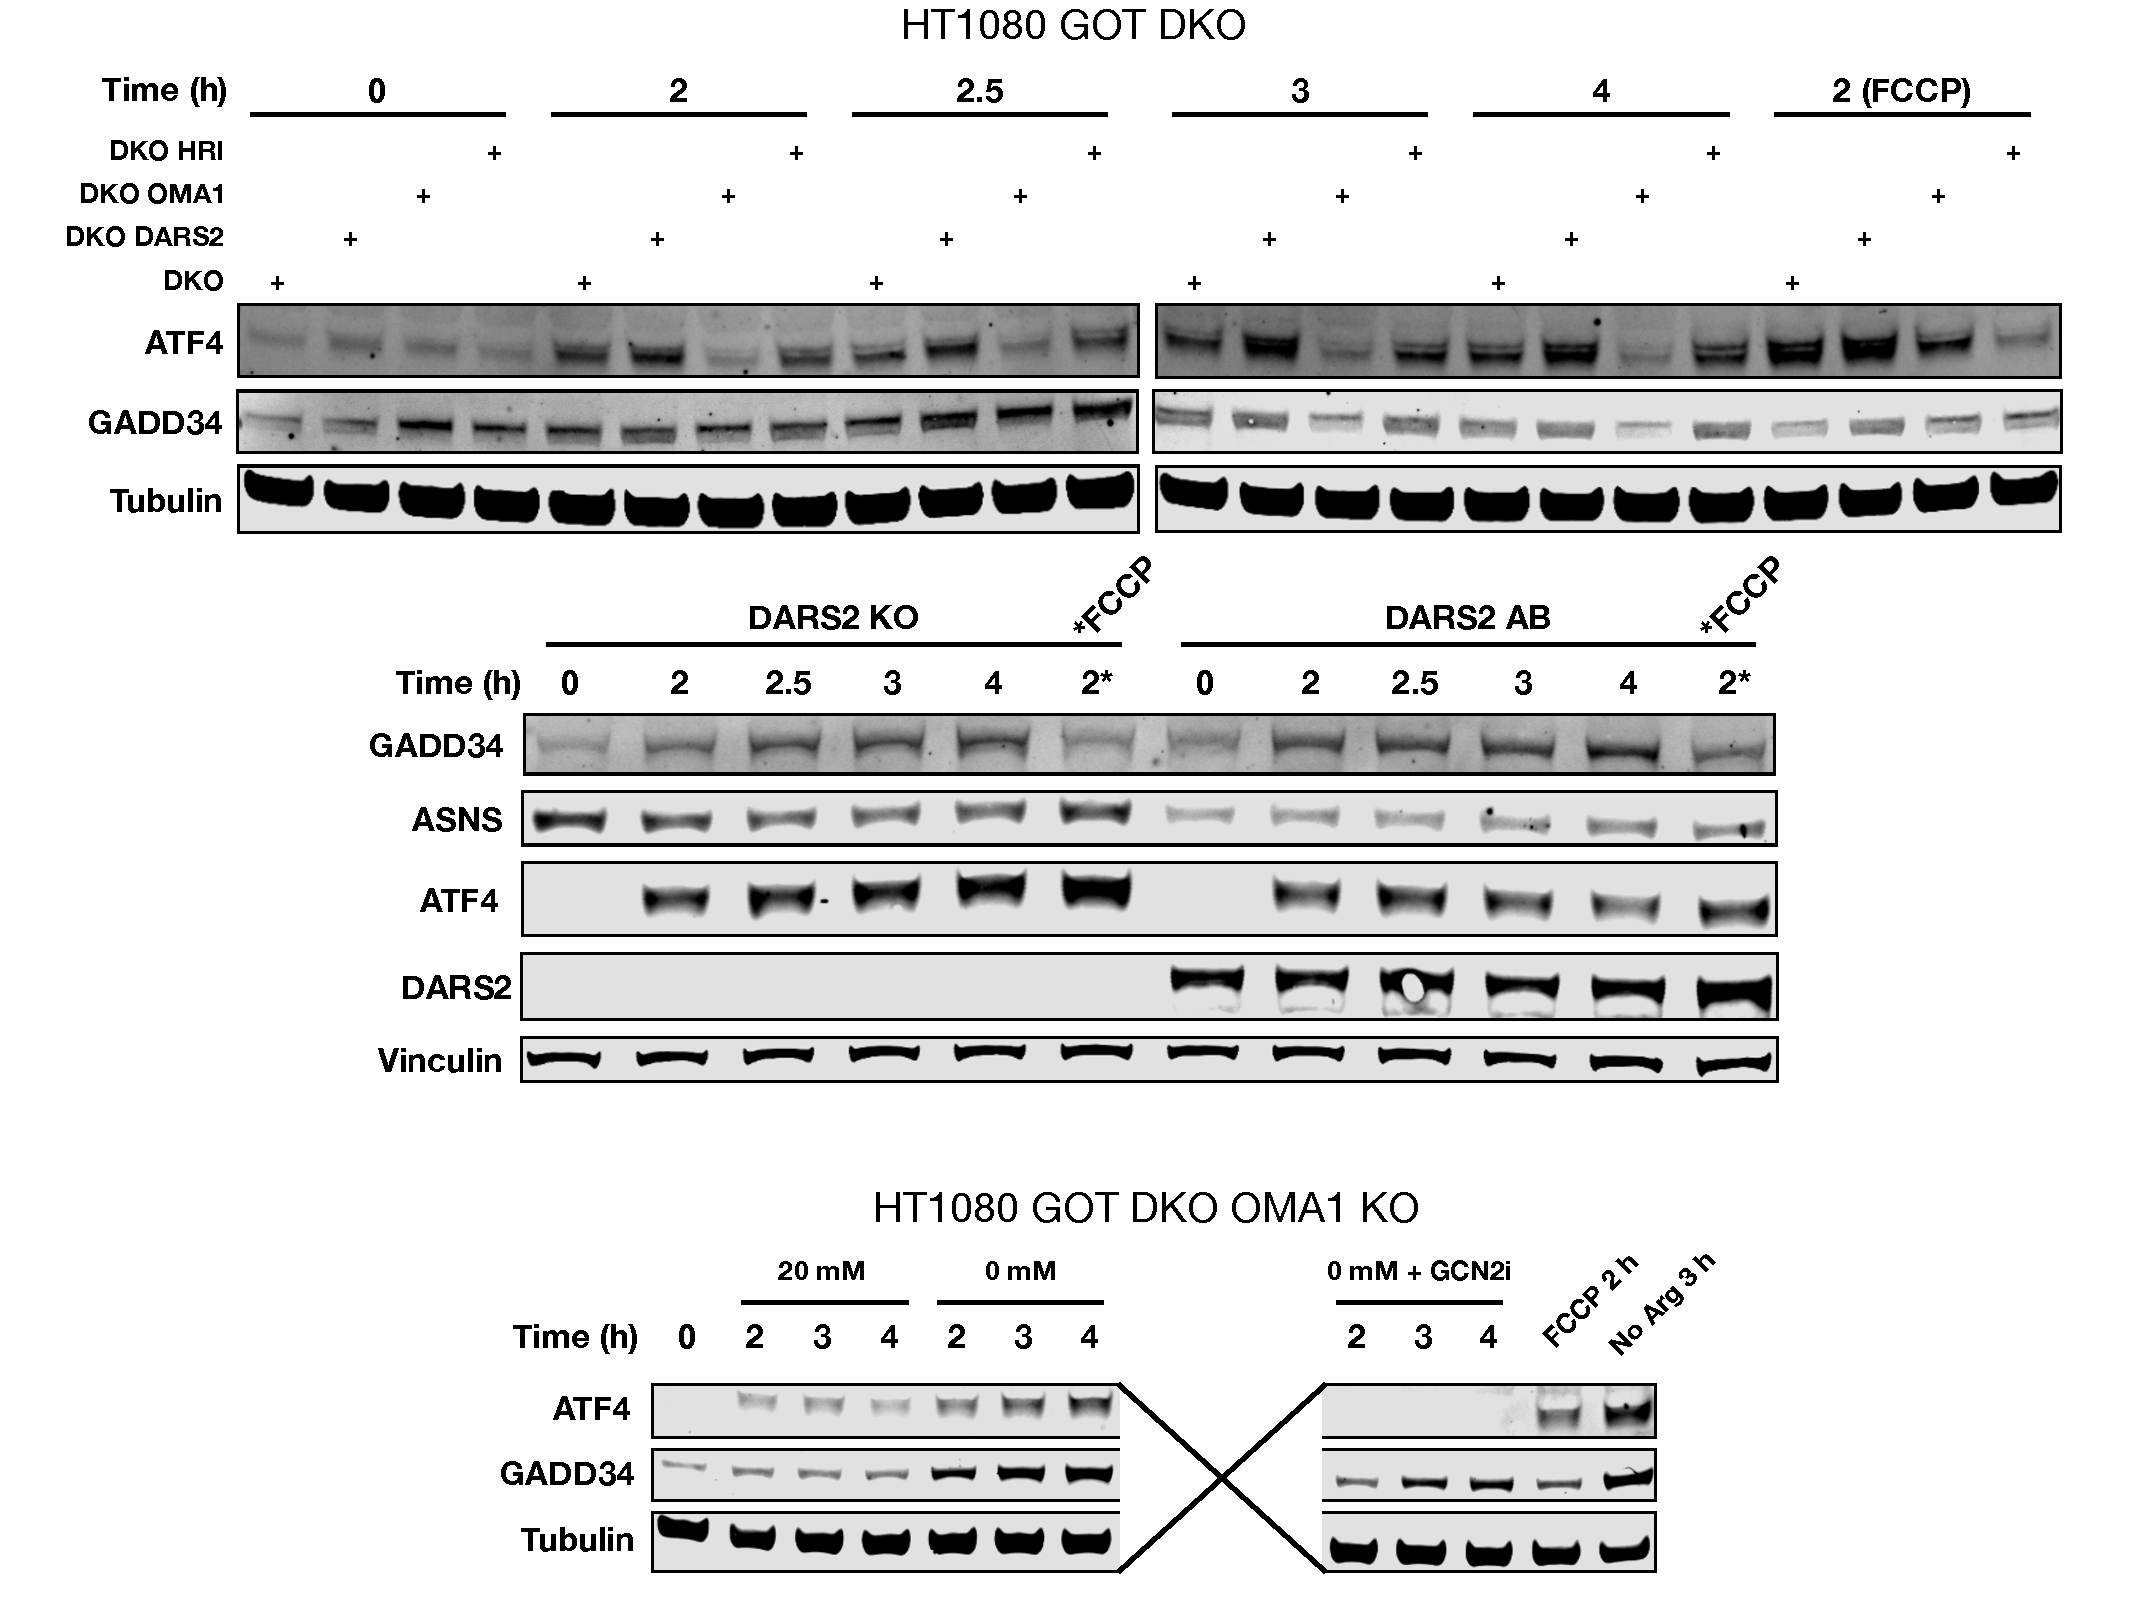
\includegraphics[width=0.95\textwidth]{figures/sapp/ISR/HT1080_DKO_KO_ISR.pdf}
    \caption[ATF4 post Asp depl. OMA1/HRI KO, western]{
    Effect of OMA1, HRI or DARS2 KO on aspartate depletion induced ISR.
    Single cell clones validated for OMA1 and DARS2, only functionally validated for HRI, see figure \ref{fig:sapp:ISR:OMA1_HRI_DARS2_val}.
    Aspartate depletion initiated by switching to media with no asp at time zero.
    Irrelevant wells spliced out.
    }
    \label{fig:sapp:ISR:HT1080_DKO_KO_ISR}
\end{figure}

\begin{figure}[ht]
     \centering
     \begin{subfigure}[b]{0.49\textwidth}
         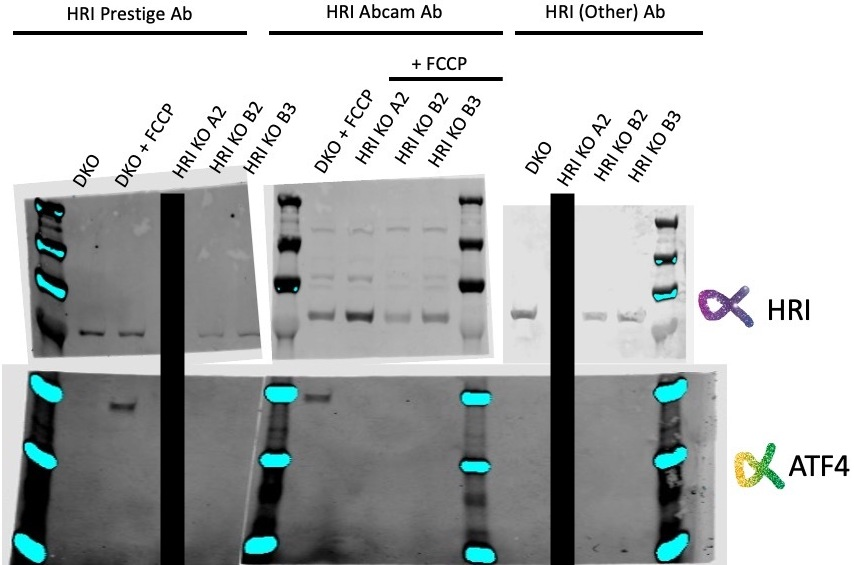
\includegraphics[width=\textwidth]{figures/sapp/ISR/HT1080_GOT_DKO_HRI_KO.jpeg}
         \caption{HT1080 GOT DKO, HRI KO}
         \label{fig:sapp:ISR:HT1080_GOT_DKO_HRI_KO}
     \end{subfigure}
     \hfill
     \begin{subfigure}[b]{0.49\textwidth}
         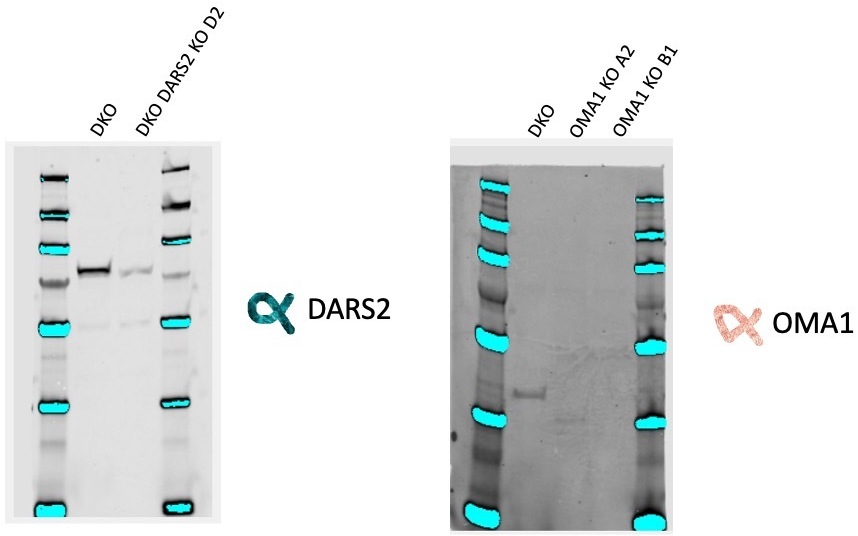
\includegraphics[width=\textwidth]{figures/sapp/ISR/HT1080_GOT_DKO_OMA1_DARS2_KO.jpeg}
         \caption{HT1080 GOT DKO, OMA1/DARS2 KO}
         \label{fig:sapp:ISR:HT1080_GOT_DKO_OMA1_DARS2_KO}
     \end{subfigure}
     \hfill
        \caption[HT1080 GOT DKO, OMA1/HRI/DARS2 KO validation]{
        Western blot validations of OMA1, HRI and DARS2 knockouts.
        Image art credit: Ian Engstrom.
        }
        \label{fig:sapp:ISR:OMA1_HRI_DARS2_val}
\end{figure}

\begin{figure}[!ht]
     \centering
     \begin{subfigure}[b]{0.6\textwidth}
         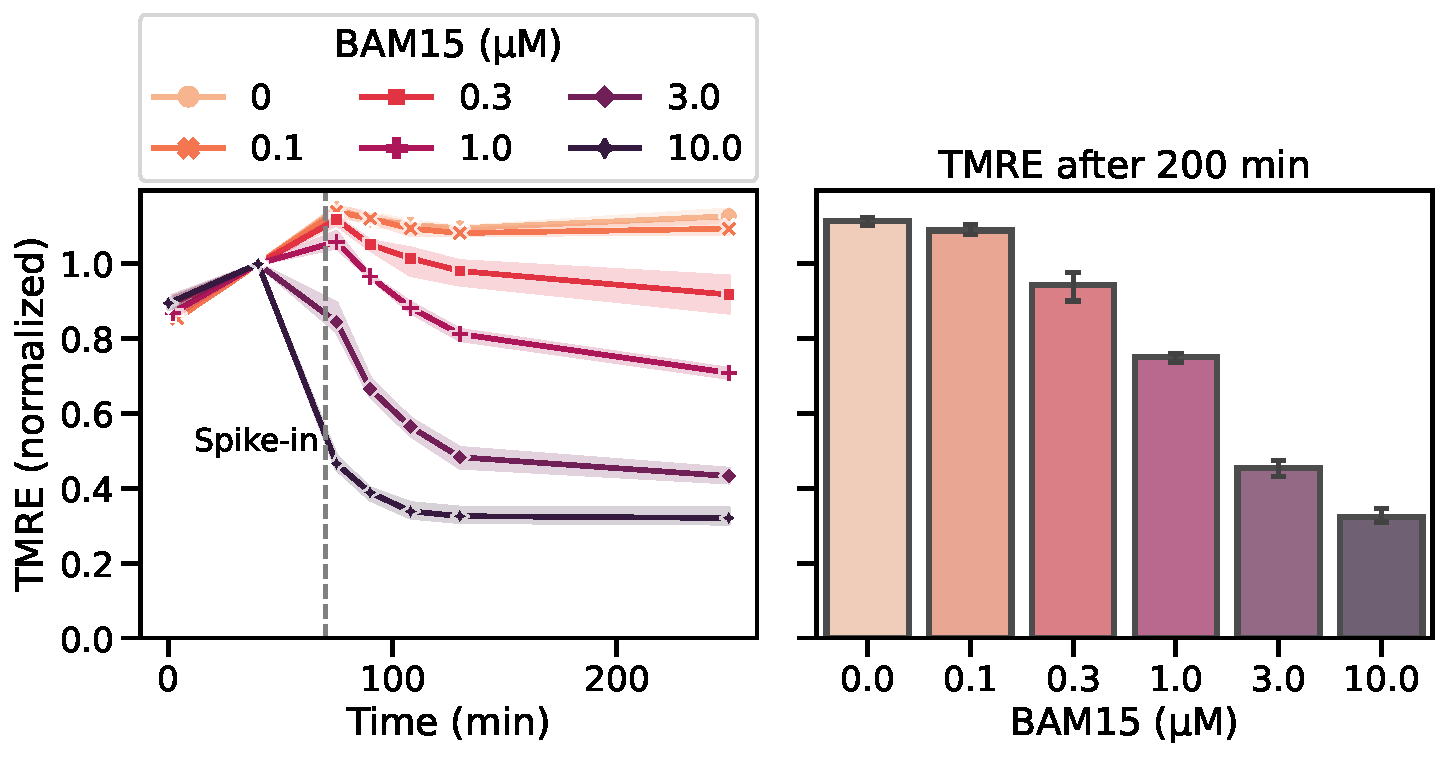
\includegraphics[width=\textwidth]{figures/sapp/ISR/HT1080_GOT_DKO_TMRA_BAM15tit.pdf}
         \caption{BAM15, mito membrane potential}
         \label{fig:sapp:ISR:HT1080_GOT_DKO_TMRA_BAM15tit}
     \end{subfigure}
     \hfill
     \begin{subfigure}[b]{0.85\textwidth}
         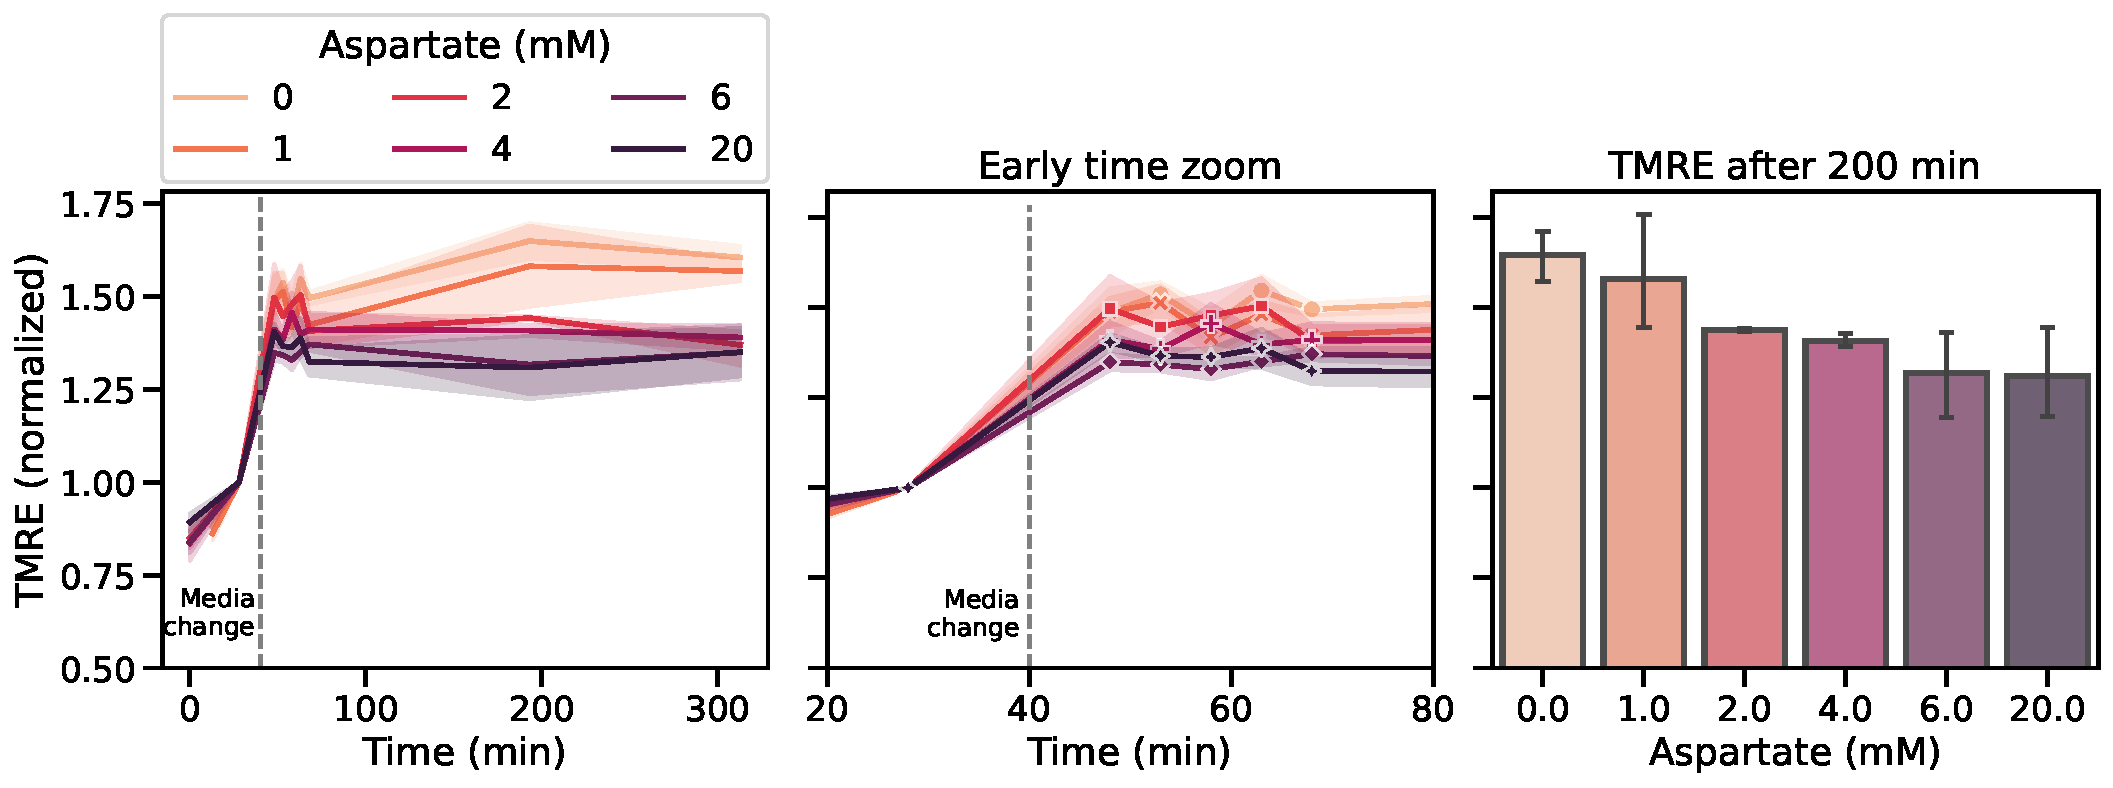
\includegraphics[width=\textwidth]{figures/sapp/ISR/HT1080_GOT_DKO_TMRA_ASPtit.pdf}
         \caption{Asp depletion, mito membrane potential}
         \label{fig:sapp:ISR:HT1080_GOT_DKO_TMRA_ASPtit}
     \end{subfigure}
     \hfill
        \caption[Mito membrane potential in GOT DKO]{
        Mitochondrial membrane potential increases slightly during aspartate depletion in HT1080 GOT DKO.
        Measured on an Incucyte using the TMRE dye.
        }
        \label{fig:sapp:ISR:HT1080_GOT_DKO_TMRE}
\end{figure}











\FloatBarrier
\subsection{ASNS over-expression to ablate rotenone/antimycin induced ISR}
If asparagine depletion is the main reason for rotenone/antimycin induced ISR maybe over-expression of ASNS would mitigate it?
Using the HT1080 ATF4 reporter cells (low baseline clone) ASNS and eGFP (control) was over-expressed using lentiviral infection.
The polyclonal population that grew out after selection was tested for ATF4 upregulation using reporter assay and western blot.
Generally, ASNS over-expression diminish ATF4 upregulation, but strangely, in this background, adding additional asparagine increase ATF4.

\begin{figure}[ht]
     \centering
     \begin{subfigure}[b]{0.49\textwidth}
         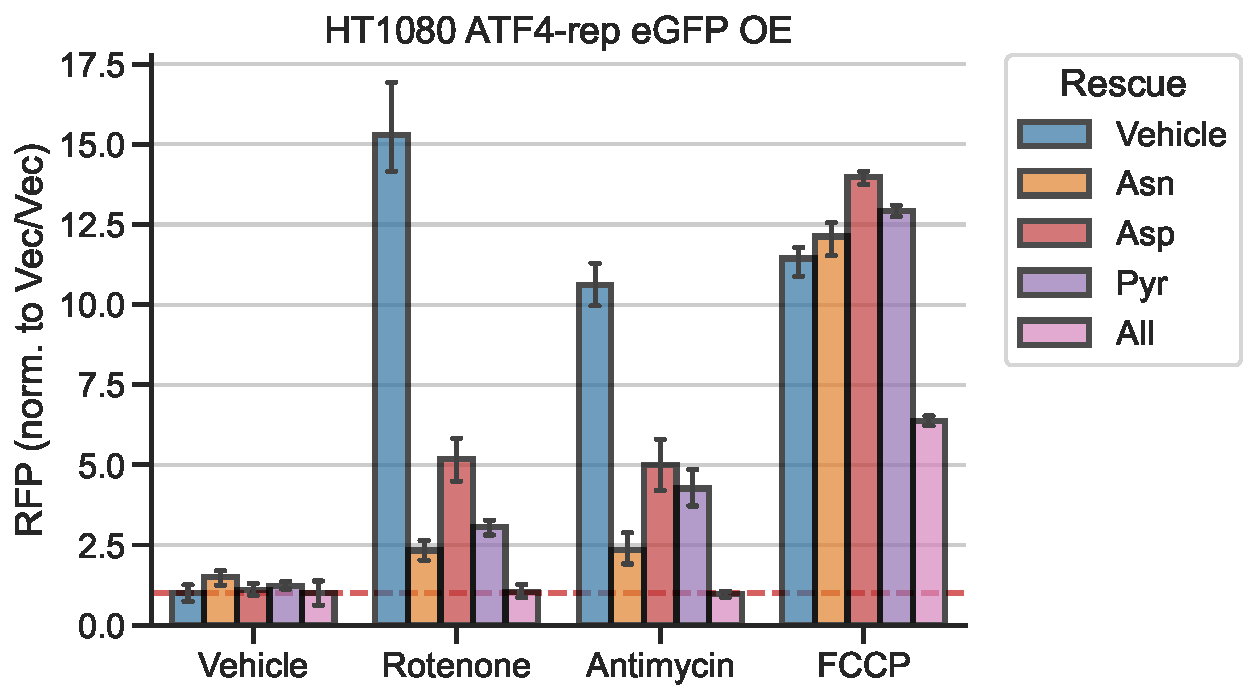
\includegraphics[width=\textwidth]{figures/sapp/ISR/HT1080_ATF4rep_eGFP_OE.pdf}
         \caption{ATF4 reporter, eGFP polyclonal}
         \label{fig:sapp:ISR:HT1080_ATF4rep_eGFP_OE}
     \end{subfigure}
     \hfill
     \begin{subfigure}[b]{0.49\textwidth}
         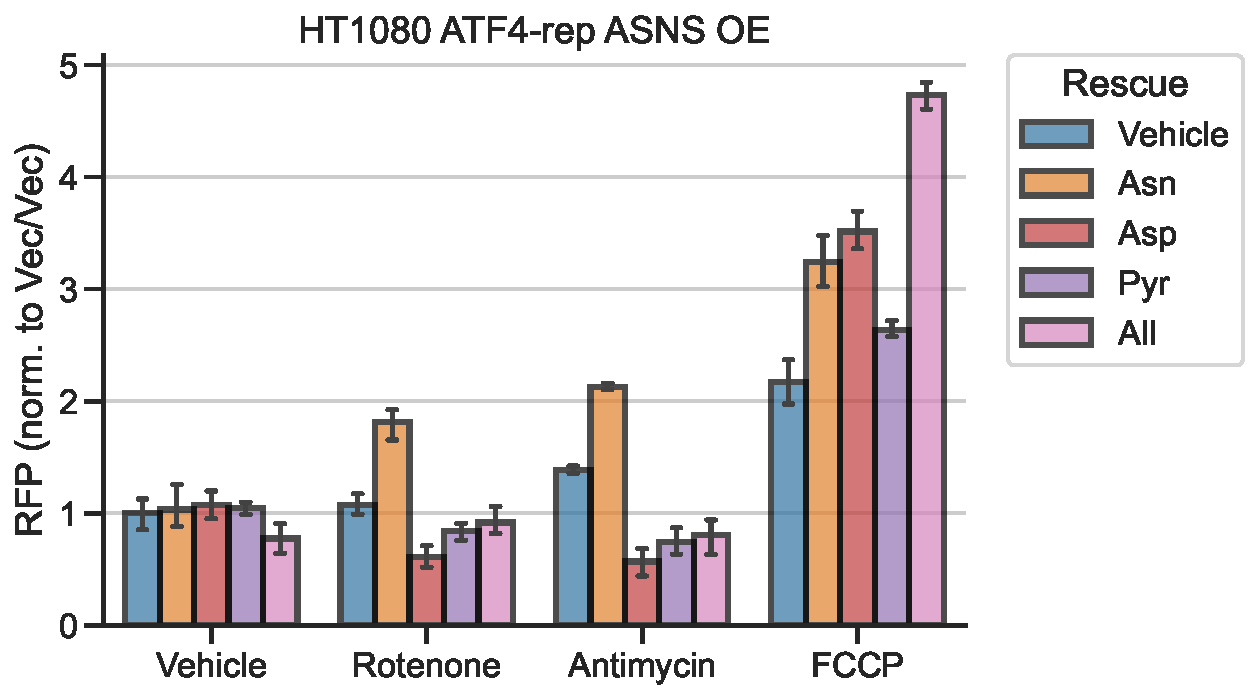
\includegraphics[width=\textwidth]{figures/sapp/ISR/HT1080_ATF4rep_ASNS_OE.pdf}
         \caption{ATF4 reporter, ASNS polyclonal}
         \label{fig:sapp:ISR:HT1080_ATF4rep_ASNS_OE}
     \end{subfigure}
     \hfill
     \begin{subfigure}[b]{0.6\textwidth}
         \centering
         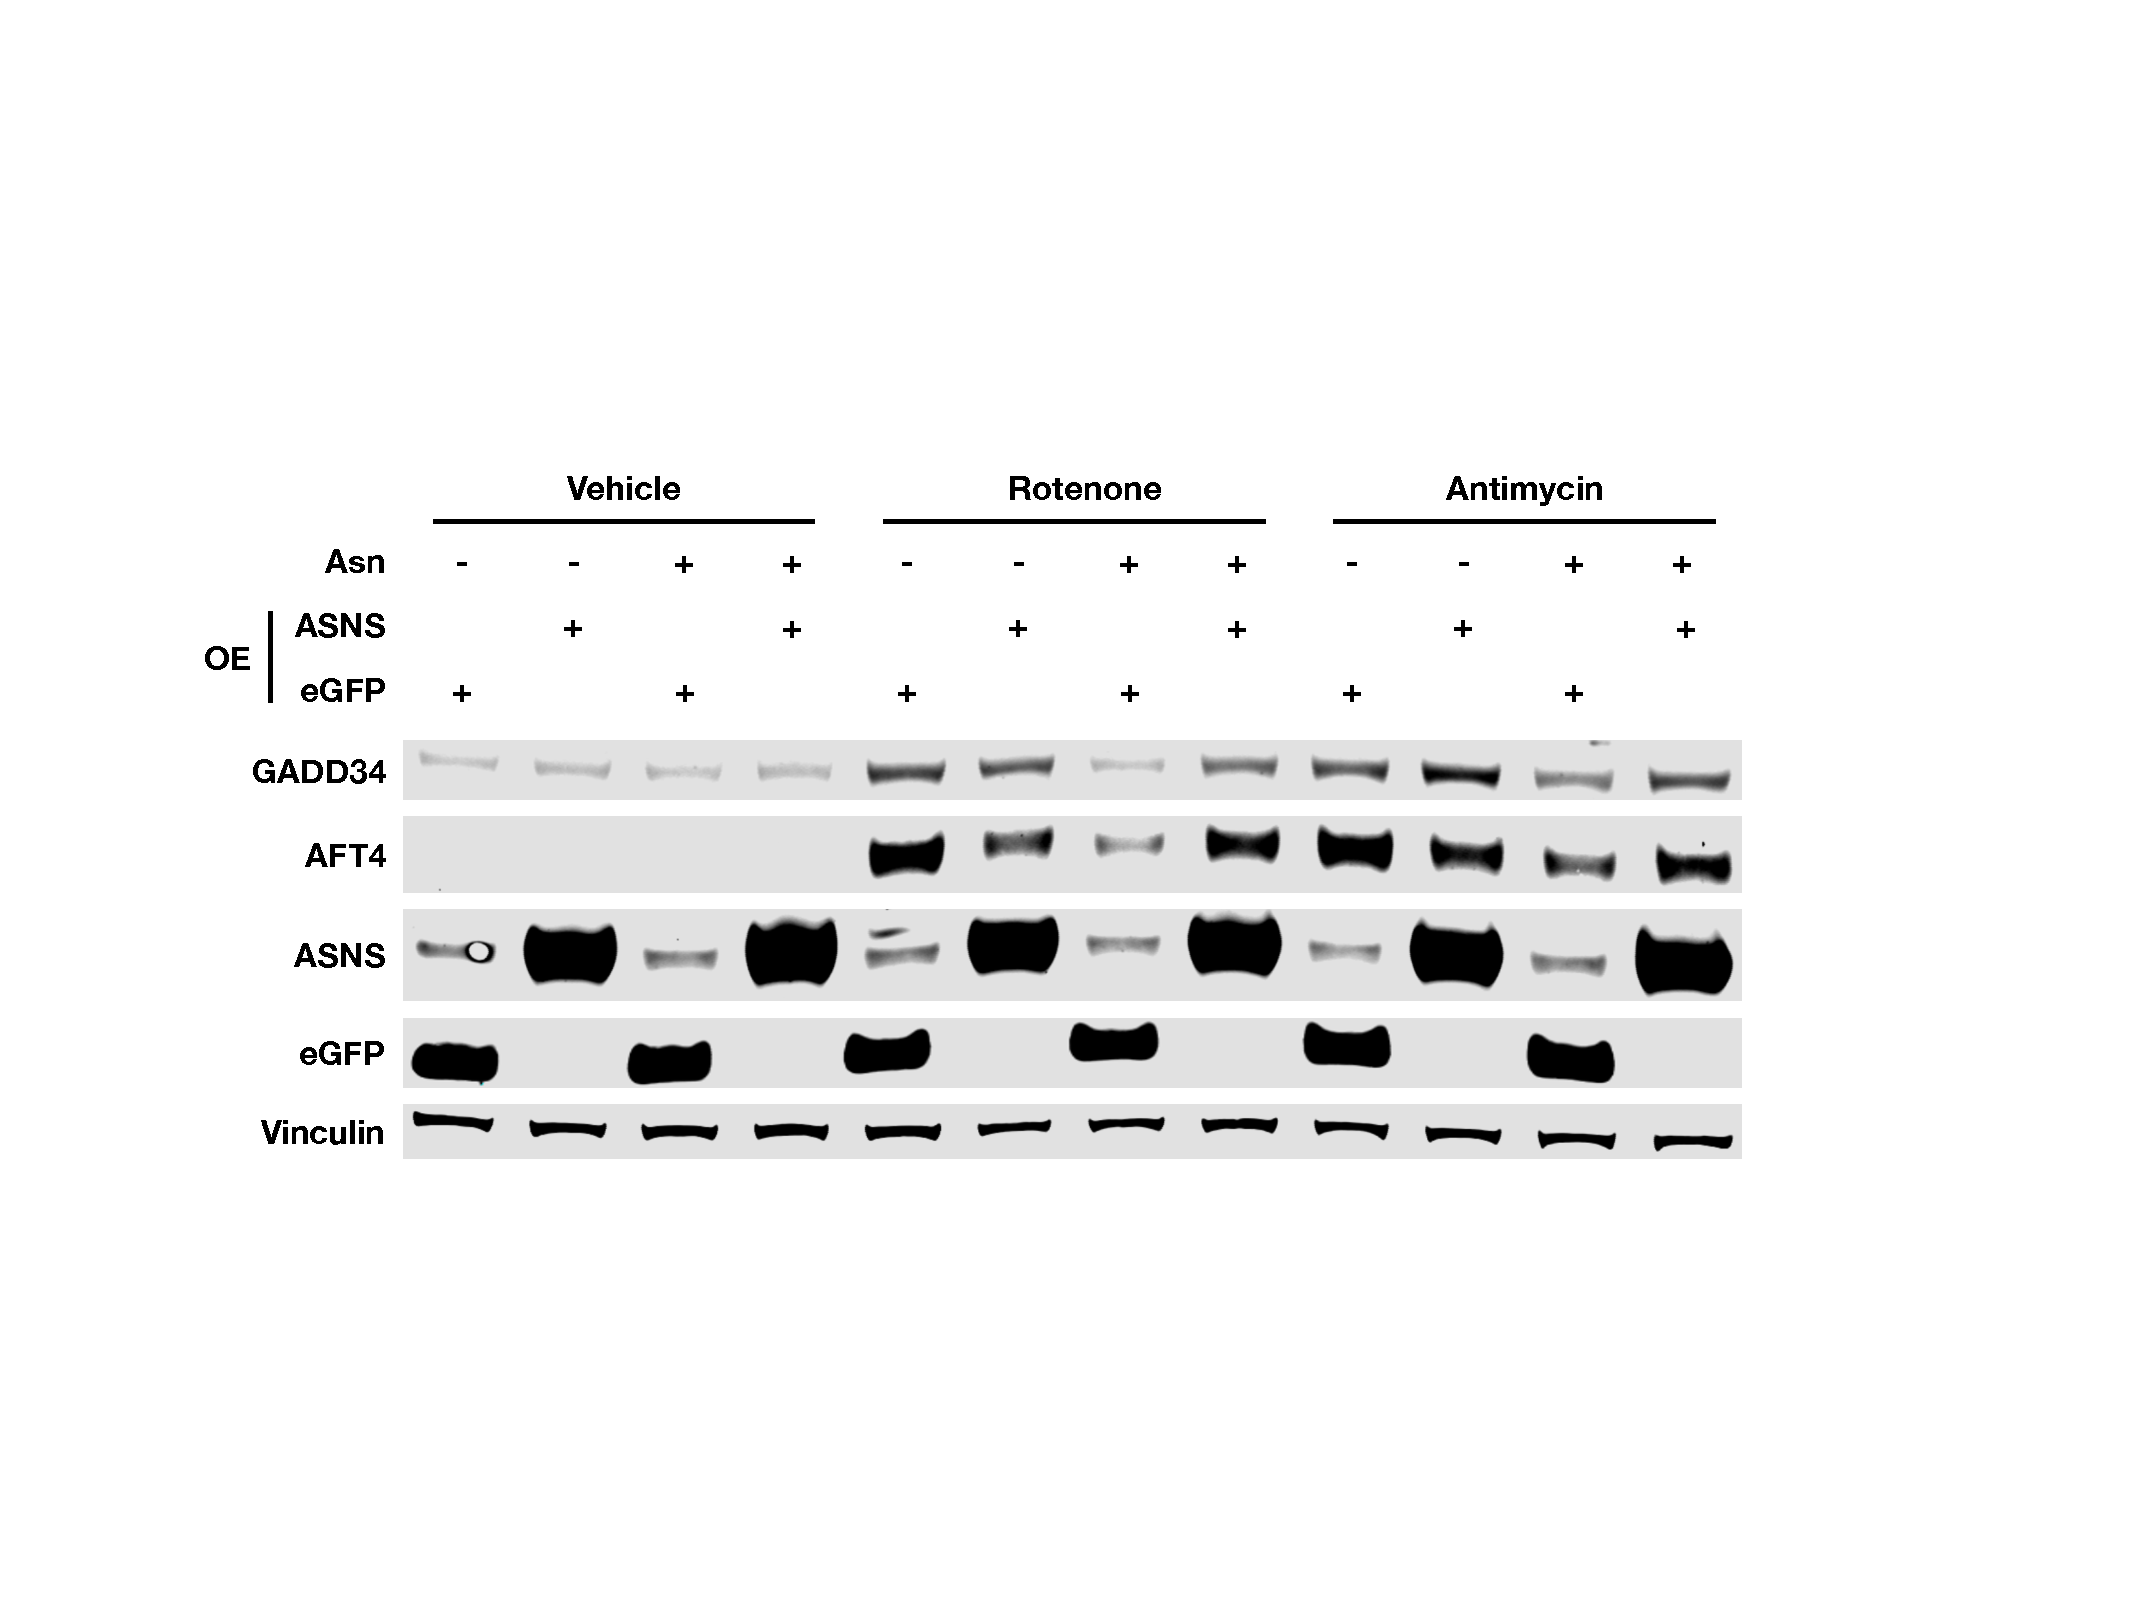
\includegraphics[width=\textwidth]{figures/sapp/ISR/HT1080_ISR_ASNS_OE.pdf}
         \caption{Western blot, eGFP/ASNS polyclonal}
         \label{fig:sapp:ISR:HT1080_ISR_ASNS_OE}
     \end{subfigure}
        \caption[ASNS OE, rotenone/antimycin induced ISR]{
        Effect of ASNS over-expression (eGFP control) on ATF4 reporter assay of ETC inhibitor induced ISR (parental HT1080 low baseline clone).
        For ATF4 reporter treatments was initiated by 10x spike-in, for western blot fresh media was added with drug at time zero.
        Using 100 nM rotenone and 1 µM antimycin.
        }
        \label{fig:sapp:ISR:ASNS_ISR}
\end{figure}







\FloatBarrier
\subsection{GCN2 relation to rotenone/antimycin induced ISR}
Now, one would think that ETC inhibitor induced ISR is induced through Asp/Asn depletion and thus mediated by GCN2 and thus a GCN2 knockout should not upregulate ATF4.
This model is what is proposed by Mick et al. \cite{Mick2020-kf} but it is only supported by one western blot showing GCN2 phosphorylation and a few experiment showing ablation of ATF4 induction when co-treating with 500 nM GCN2iB (Takeda \cite{Nakamura2018-mt}).
GCN2iB, is an ATP analog and there is conflicting evidence of its off-target tendencies.
The inventors, Nakamura et al. \cite{Nakamura2018-mt}, screens for off-target kinase inhibition but does not report specifically on related kinase HRI, PKR and PERK.
However, an AACR poster [\href{https://rapt.com/wp-content/uploads/2019/04/FLX-Bio-GCN2-poster-AACR-2019.pdf}{link}], from a competing group with their own drug \cite{Jackson2022-wv}, suggests that this and other GCN2 inhibitors have off-target effects on HRI with IC50 in the 10-500 nM range.
Thus, using 500 nM GCN2i as in Mick et al., and 2000 nM as we have done, could lead to robust GCN2 and HRI dual inhibition and mask any effect from HRI.
A GCN2 knockout would be a better way to differentiate the two.

We only have a confirmed GCN2 knockout in 293T cells and therefore tried with these.
Strangely, ISR in 293T cells was not reverted well with Asp/Asn, but even more strange the GCN2 KO cells did not have ablated ATF4.

\begin{figure}[ht]
    \centering
    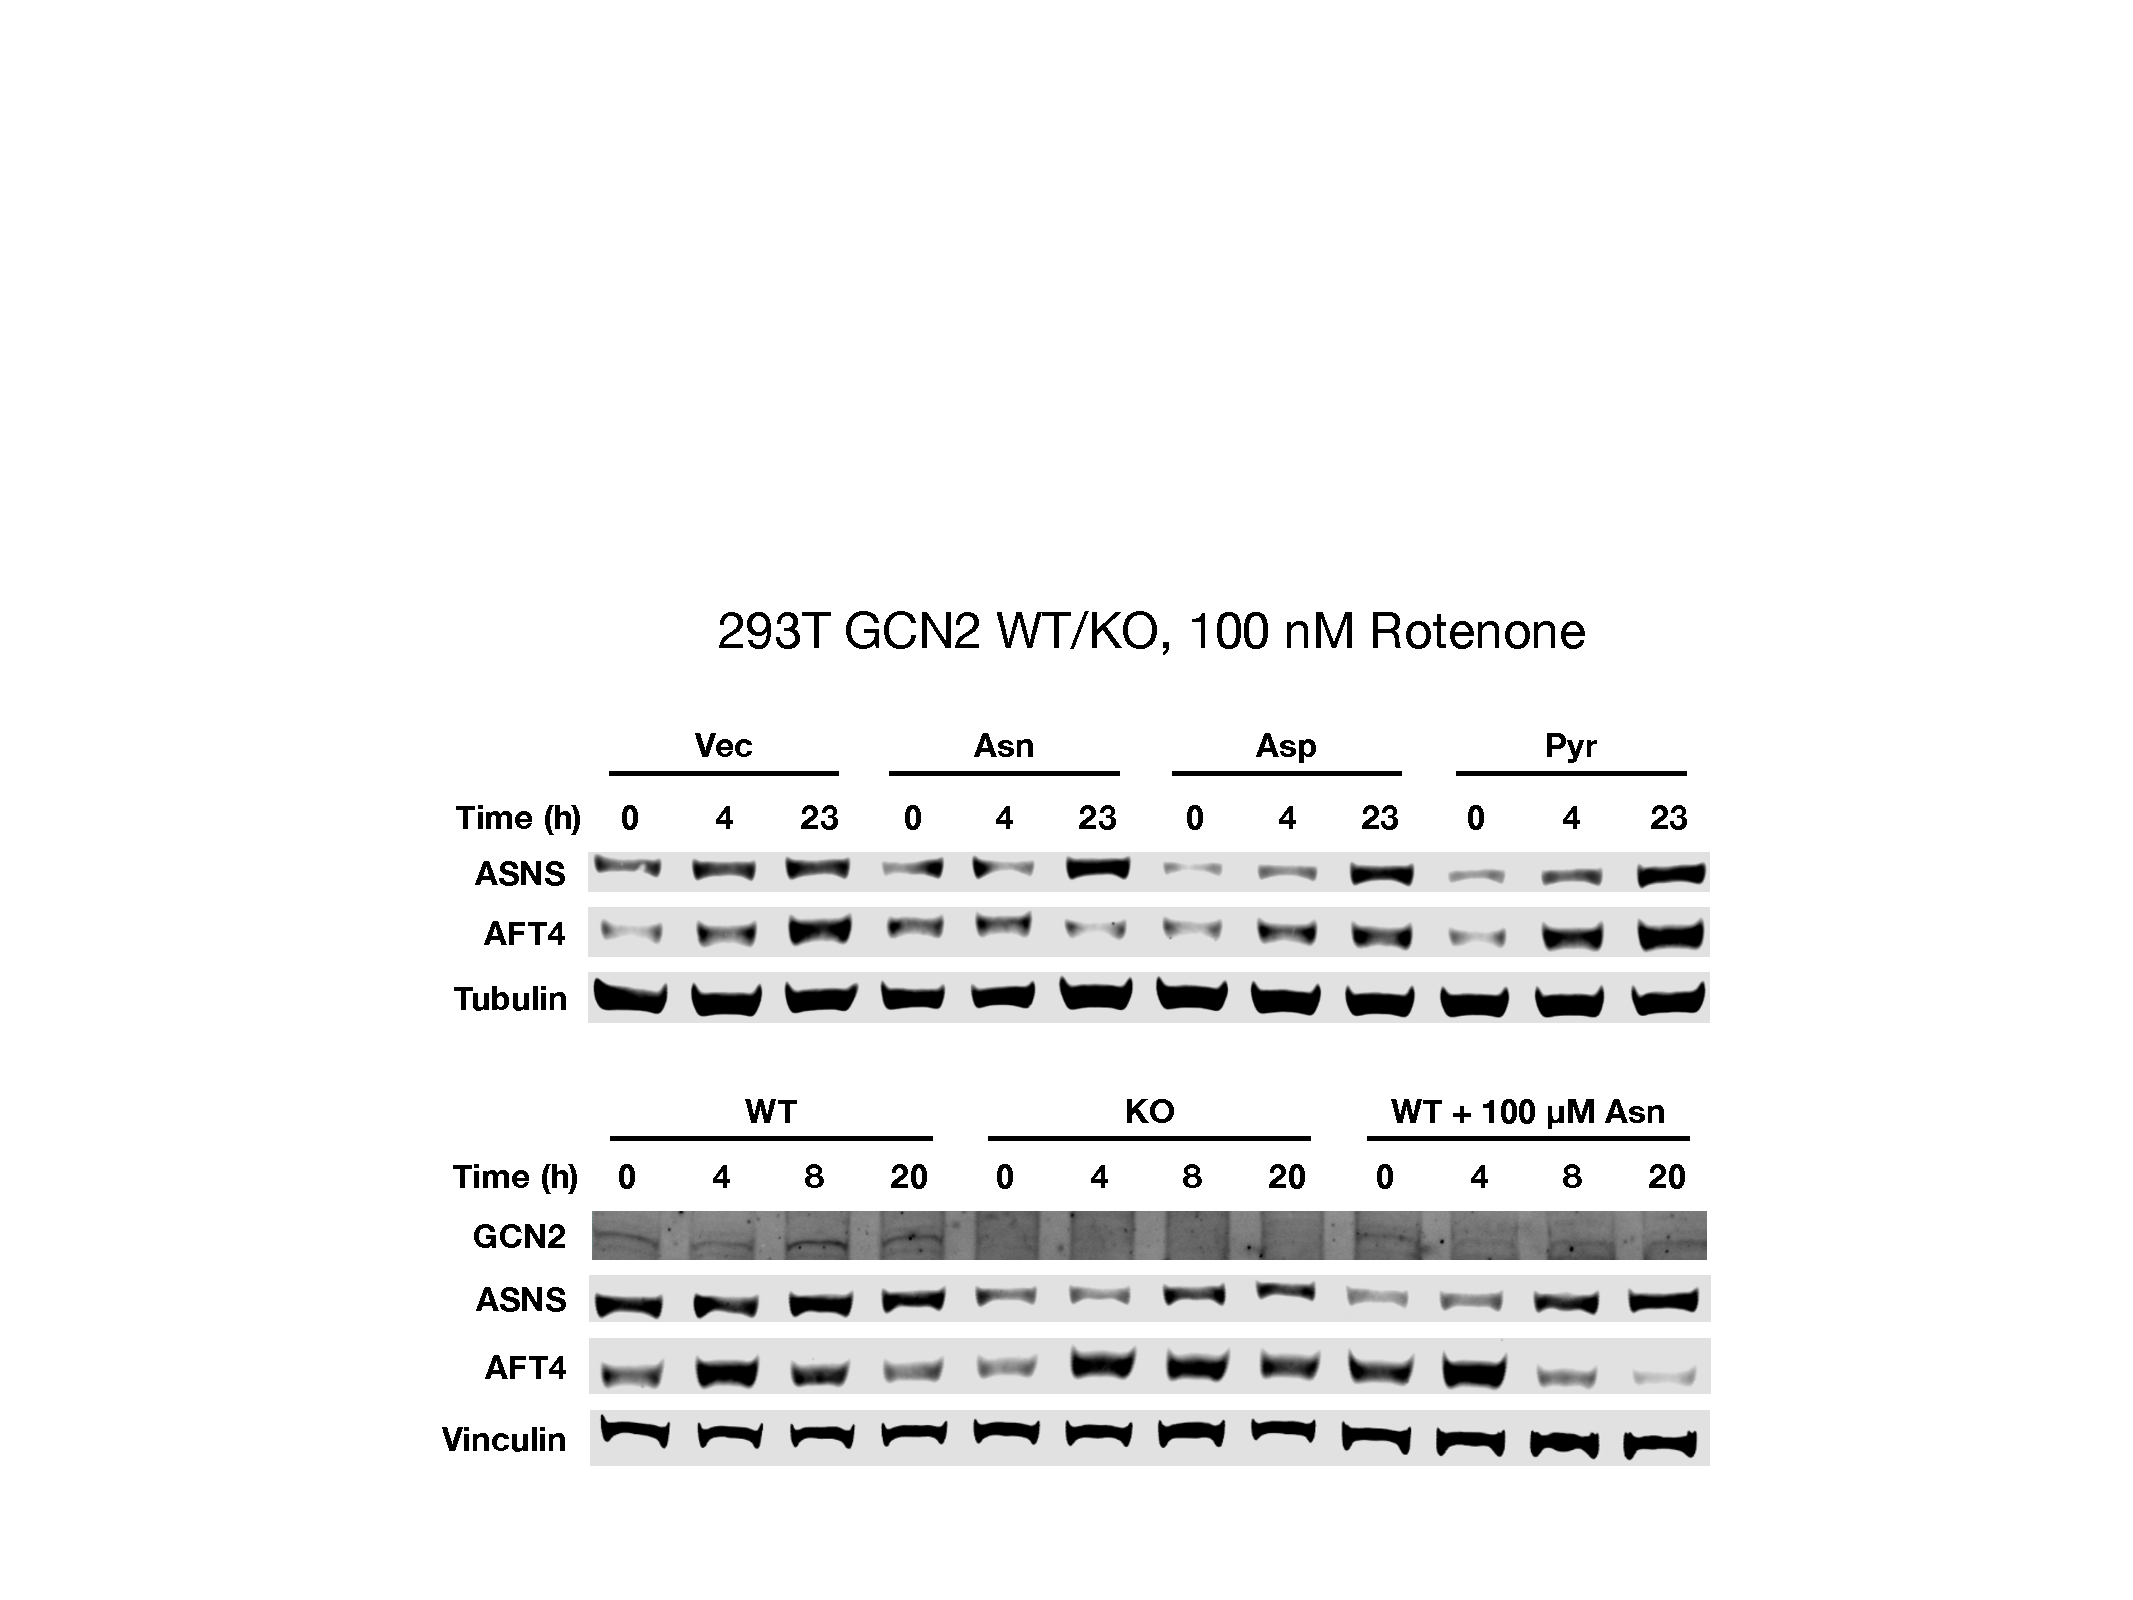
\includegraphics[width=0.70\textwidth]{figures/sapp/ISR/293T_GCN2_ISR.pdf}
    \caption[ATF4 post mito inhib. GCN2 KO, western]{
    Rotenone treatment was initiated by adding fresh media with 100 nM rotenone at time zero.
    Rescue conditions: Asn (500 µM), Asp (30 mM) or Pyr (2 mM) was also added to media >1 h before time zero.
    Top, WT with different rescues.
    Bottom WT vs. GCN2 KO.
    }
    \label{fig:sapp:ISR:293T_GCN2_ISR}
\end{figure}


\FloatBarrier
We have pooled knockout cells (parental 143B ATF4 reporter high clone) of GCN2 that also maintain Asn rescuable ATF4 induction upon rotenone/antimycin treatment.
Monoclonal knockouts were never isolated due to the difficulty of GCN2 detection on western blots; however, the knockout protocol is typically very efficient.
Taking these data at face value, GCN2 is not required for rotenone/antimycin induced ISR.

\begin{figure}[ht]
    \centering
    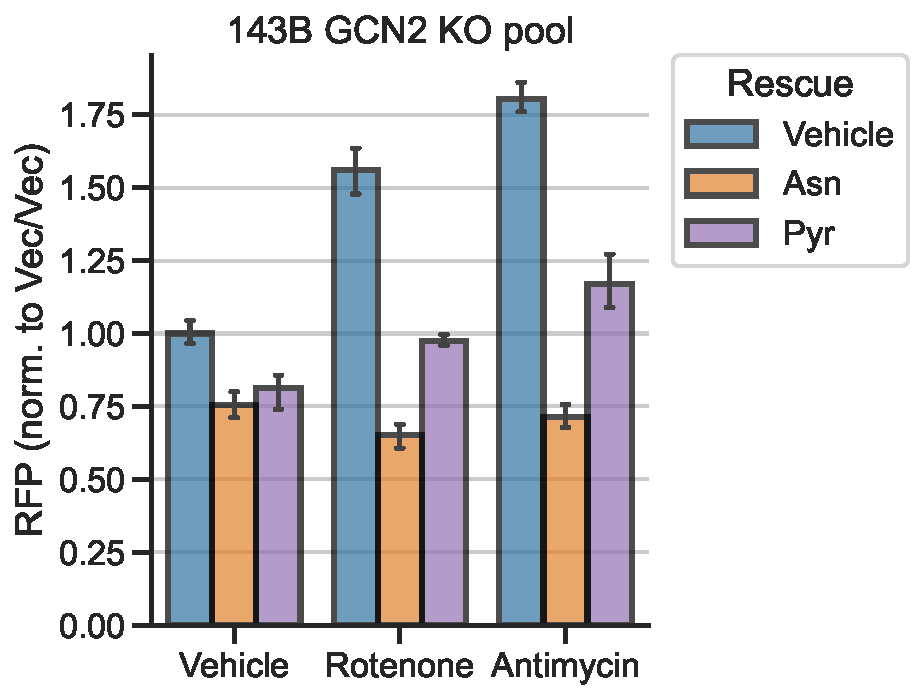
\includegraphics[width=0.55\textwidth]{figures/sapp/ISR/143B_GCN2_ISR.pdf}
    \caption[ATF4 post mito inhib. GCN2 KO, reporter]{
    ATF4 reporter assay measured 21 h after drug treatment with vehicle, rotenone (100 nM) or antimycin (1 µM) spiked-in as 10x.
    }
    \label{fig:sapp:ISR:143B_GCN2_ISR}
\end{figure}






\FloatBarrier
\section{tRNA charge changes}
Supposedly, GCN2 phosphorylation is stimulated by uncharged tRNAs \cite{Wek1989-yw, Dong2000-si}, or ribosome collisions \cite{Harding2019-kb, Wu2020-lq, Yan2021-yv}, the latter explaining GCN2 activation upon UV radiation.
Measuring the tRNA charge effect of ISR inducing, aspartate depleting treatments, such as electron chain inhibitors, would be a good confirmation of whether ISR is driven by GCN2.

First, in 143B cell a high dose antimycin is spiked-in and tRNA charge followed over time (figure \ref{fig:sapp:tRNA:143B_Anti_time}).
Cytoplasmic tRNA\textsuperscript{Asp} remain charged throughout the time-course, but cytoplasmic tRNA\textsuperscript{Asn} starts to decrease after $\sim$9 hours.
Of note, the discontinuity of cyto-tRNA\textsuperscript{Asn} charge between 12 and 15 hours is likely due to sampling artifacts.
For practical reasons the 12 hour timepoint was spiked at 8:00 and harvested at 20:00 whereas the 15 hour timepoint was spiked at 19:00 and harvested the next day at 10:00.
This time difference would likely lead to higher media asparagine concentration due to cellular efflux, which would would then buffer the decrease in cyto-tRNA\textsuperscript{Asn} charge.
Regardless, mito-tRNA\textsuperscript{Asn} charge is rapidly decreasing in a timeframe that is compatible with the induction of ISR that happens within 1-2 hours.
Decreased charge of cyto-tRNA\textsuperscript{Asn} is not compatible with the early induction of ISR but it is with a later induction.
Thus, ISR may be induced two-fold - first an early GCN2 independent induction, and then a GCN2 dependent induction caused by uncharged cyto-tRNA\textsuperscript{Asn}.





The resulting eIF2alpha phosphorylation causes a global decrease in protein synthesis
Glu codon
.




\begin{figure}[!ht]
     \centering
     \begin{subfigure}[b]{0.6\textwidth}
         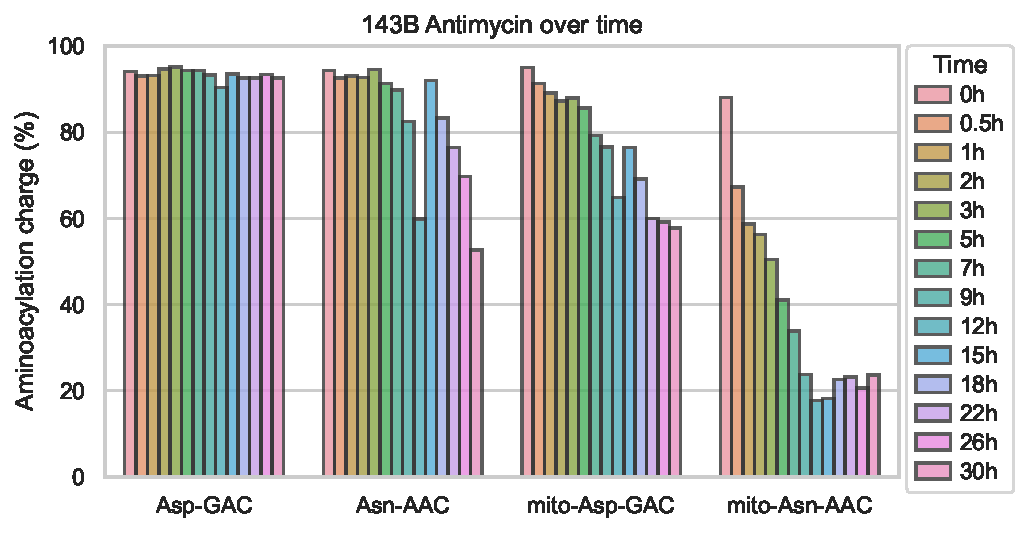
\includegraphics[width=\textwidth]{figures/sapp/tRNA/143B_Anti-time_Asp-Asn.pdf}
     \end{subfigure}
     \begin{subfigure}[b]{0.7\textwidth}
         \vspace{5pt}
         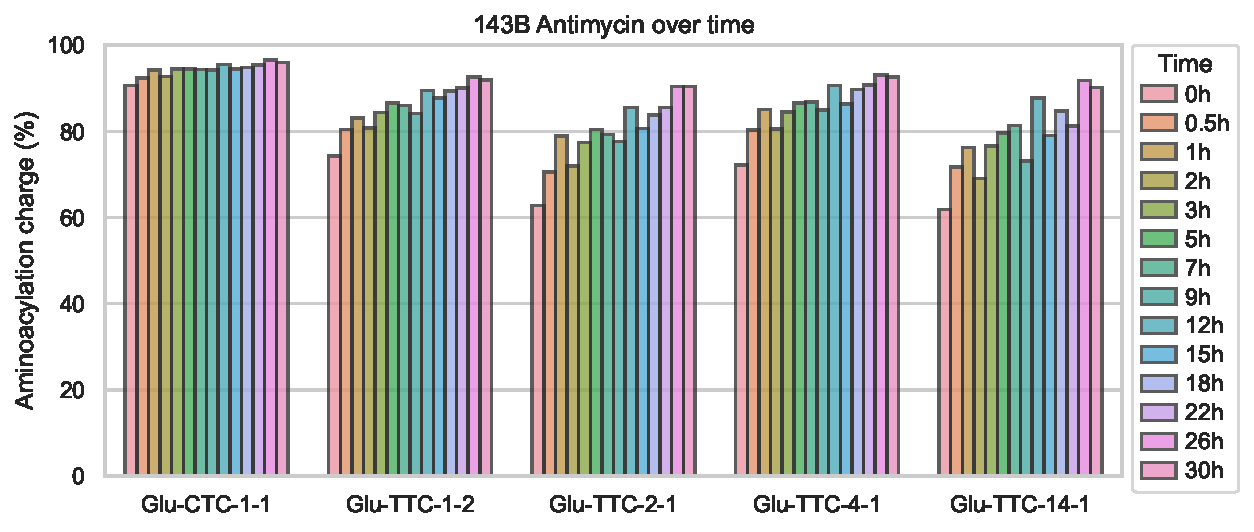
\includegraphics[width=\textwidth]{figures/sapp/tRNA/143B_Anti-time_Glu.pdf}
     \end{subfigure}
     \hfill
        \caption[Antimycin time-series in 143B, effect on tRNA charge]{
        tRNA charge as a function of time after antimycin treatment (1 µM spike-in) of 143B cells in DMEM, without pyruvate, with dialyzed FBS and 200 µM uridine.
        Top panel, effect on aspartate and asparagine tRNA charge.
        Bottom panel, effect on cytoplasmic glutamate codons with TTC charge being a potential marker inversely correlated with translation.
        For other tRNAs (cytoplasmic as well as mitochondrial) antimycin inhibitors had little or insignificant effect on charge.
        }
        \label{fig:sapp:tRNA:143B_Anti_time}
\end{figure}




\begin{figure}[!ht]
     \centering
     \begin{subfigure}[b]{0.6\textwidth}
         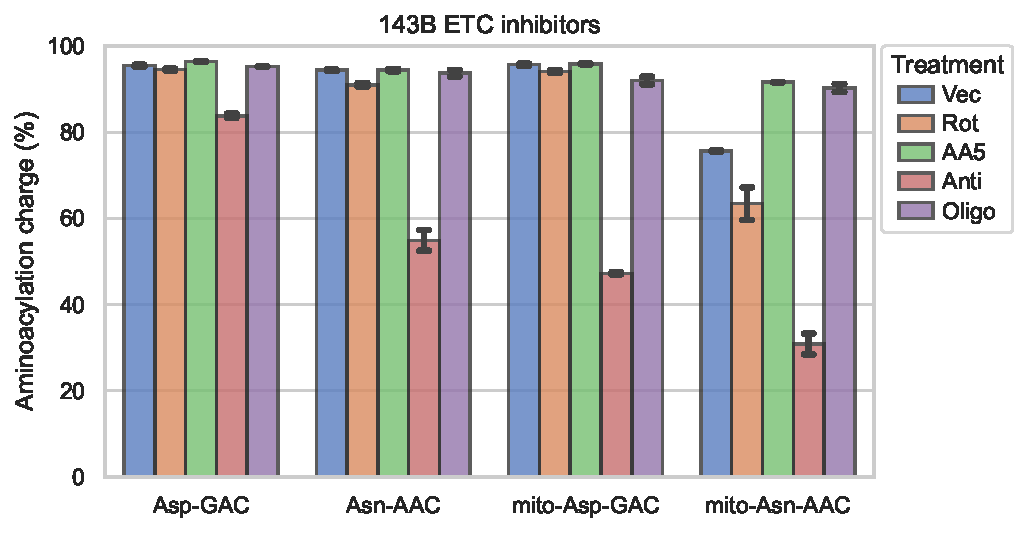
\includegraphics[width=\textwidth]{figures/sapp/tRNA/143B_ETCinhib_Asp-Asn.pdf}
     \end{subfigure}
     \begin{subfigure}[b]{0.8\textwidth}
         \vspace{5pt}
         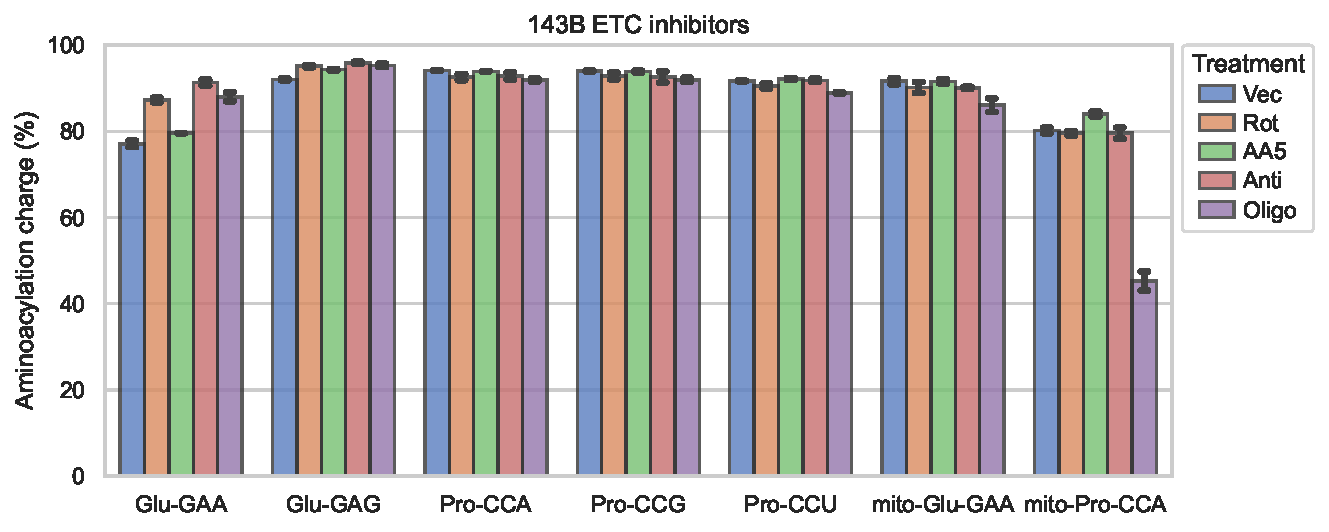
\includegraphics[width=\textwidth]{figures/sapp/tRNA/143B_ETCinhib_Glu-Pro.pdf}
     \end{subfigure}
     \hfill
        \caption[ETC inhibitor in 143B, effect on tRNA charge]{
        tRNA charge after 30 hours treatment with vehicle, rotenone (50 nM), atpenin (5 µM), antimycin (0.5 µM) or oligomycin (0.25 µM).
        For all treatments cells were grown in DMEM, without pyruvate, with dialyzed FBS.
        For antimycin and oligomycin treatments, 200 µM uridine was added to the media.
        For the atpenin treatment, 1 mM pyruvate was added to the media.
        For other tRNAs (cytoplasmic as well as mitochondrial) ETC inhibitors had little or insignificant effect on charge.
        }
        \label{fig:sapp:tRNA:143B_ETCinhib}
\end{figure}





\begin{figure}[!ht]
     \centering
     \begin{subfigure}[b]{0.6\textwidth}
         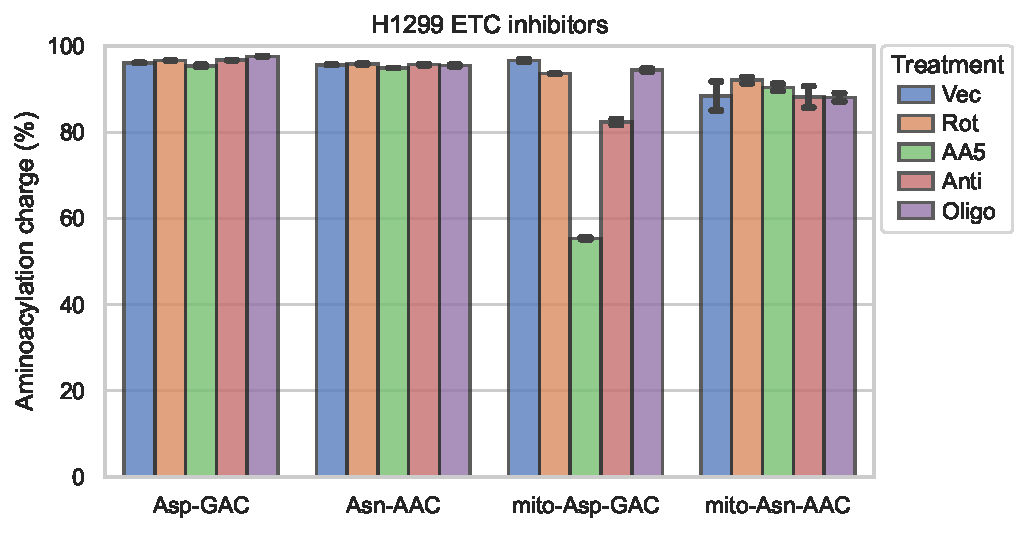
\includegraphics[width=\textwidth]{figures/sapp/tRNA/H1299_ETCinhib_Asp-Asn.pdf}
     \end{subfigure}
     \begin{subfigure}[b]{0.8\textwidth}
         \vspace{5pt}
         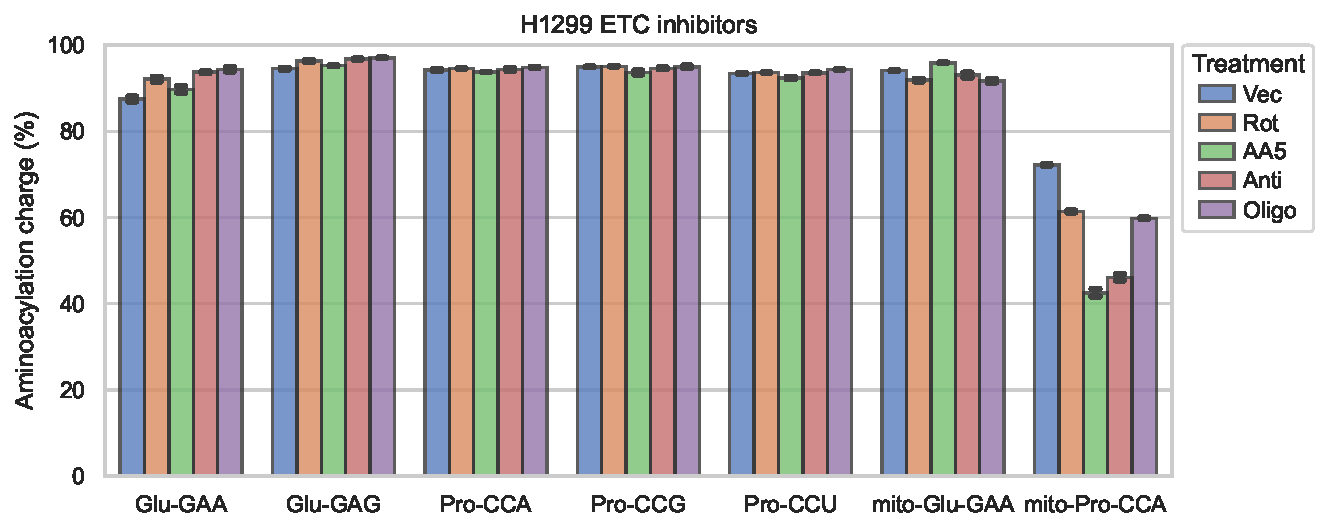
\includegraphics[width=\textwidth]{figures/sapp/tRNA/H1299_ETCinhib_Glu-Pro.pdf}
     \end{subfigure}
     \hfill
        \caption[ETC inhibitor in H1299, effect on tRNA charge]{
        tRNA charge after 30 hours treatment with vehicle, rotenone (100 nM), atpenin (5 µM), antimycin (5 µM) or oligomycin (1 µM).
        For all treatments cells were grown in DMEM, without pyruvate, with dialyzed FBS.
        For antimycin and oligomycin treatments, 200 µM uridine was added to the media.
        For the atpenin treatment, 1 mM pyruvate was added to the media.
        For other tRNAs (cytoplasmic as well as mitochondrial) ETC inhibitors had little or insignificant effect on charge.
        }
        \label{fig:sapp:tRNA:H1299_ETCinhib}
\end{figure}











\begin{figure}[!ht]
     \centering
     \begin{subfigure}[b]{0.7\textwidth}
         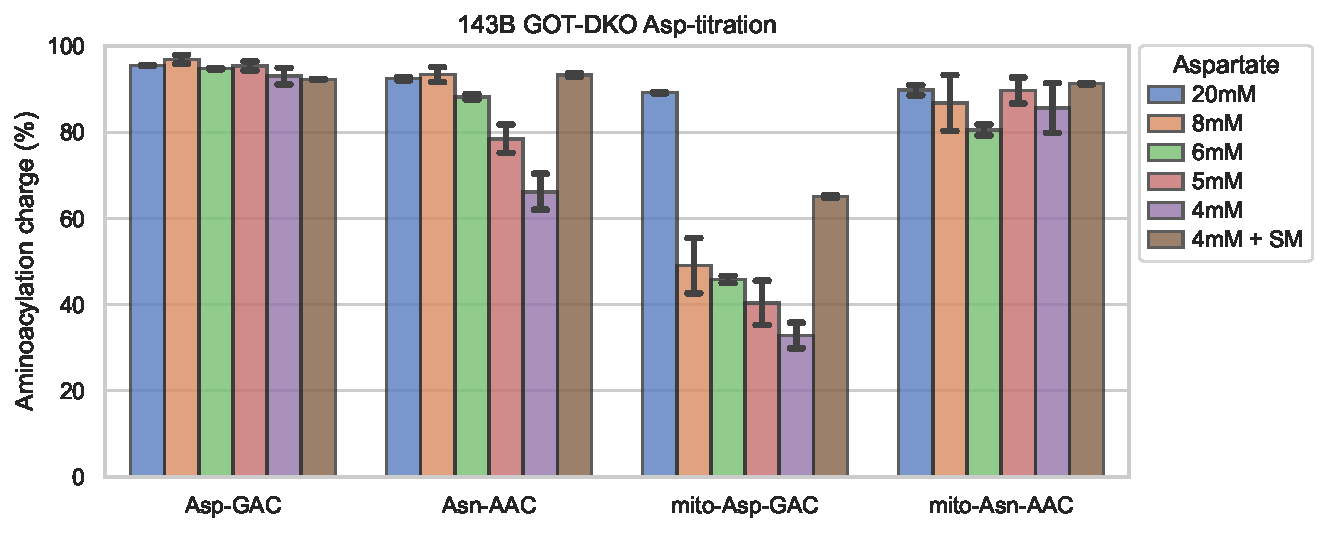
\includegraphics[width=\textwidth]{figures/sapp/tRNA/143B-DKO_Asp-Asn.pdf}
     \end{subfigure}
     \begin{subfigure}[b]{0.7\textwidth}
         \vspace{5pt}
         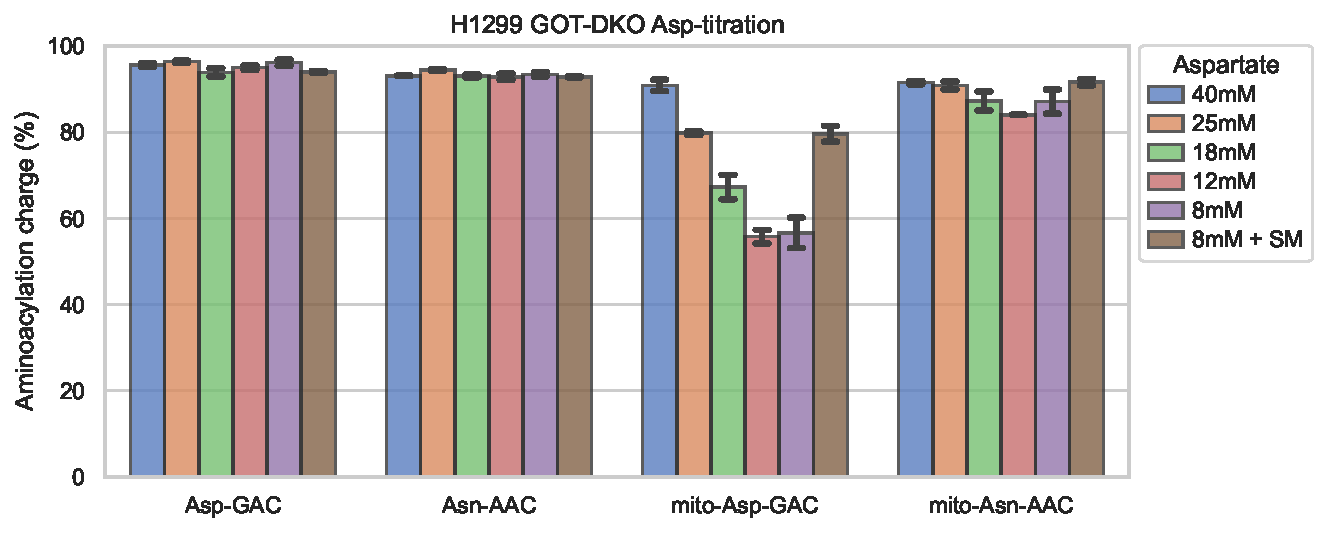
\includegraphics[width=\textwidth]{figures/sapp/tRNA/H1299-DKO_charge_Asp-Asn.pdf}
     \end{subfigure}
     \begin{subfigure}[b]{0.7\textwidth}
         \vspace{5pt}
         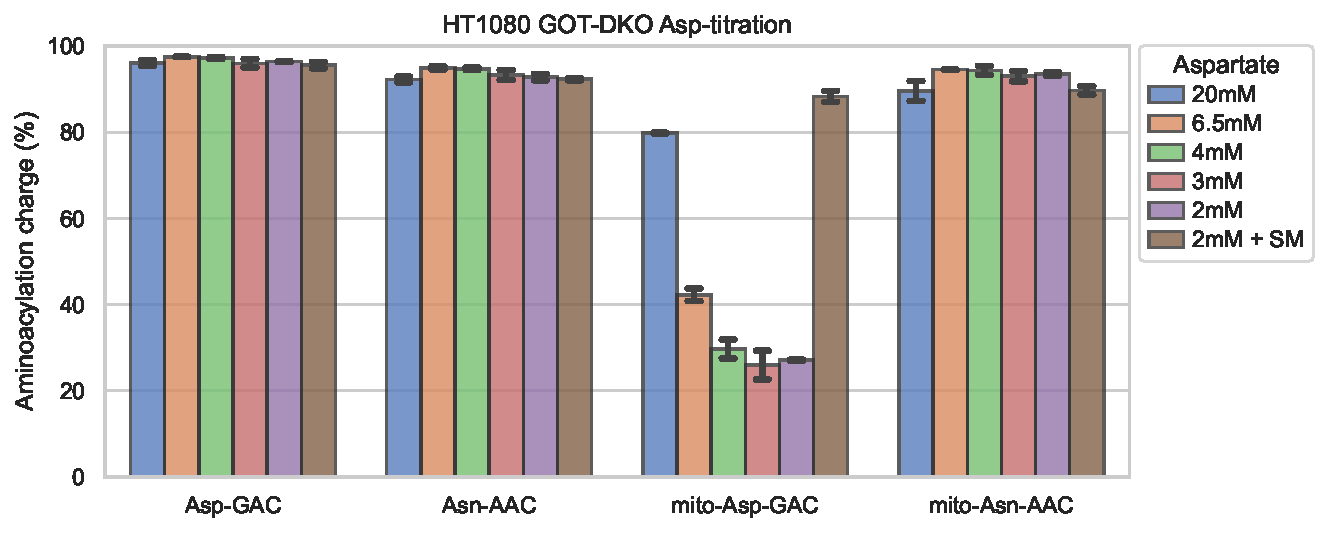
\includegraphics[width=\textwidth]{figures/sapp/tRNA/HT1080-DKO_charge_Asp-Asn.pdf}
     \end{subfigure}
     \hfill
        \caption[tRNA charge in GOT DKO Asp-tit]{
        tRNA charge as a function of media aspartate concentration.
        Conditions with salvage mix (SM) contain: 500 µM asparagine, 200 µM uridine and 100 µM adenine.
        For other tRNAs (cytoplasmic as well as mitochondrial) aspartate titration had insignificant effect on charge.
        }
        \label{fig:sapp:tRNA:DKO_Asp-Asn}
\end{figure}


Put proliferation data here.




\begin{figure}[ht]
    \centering
    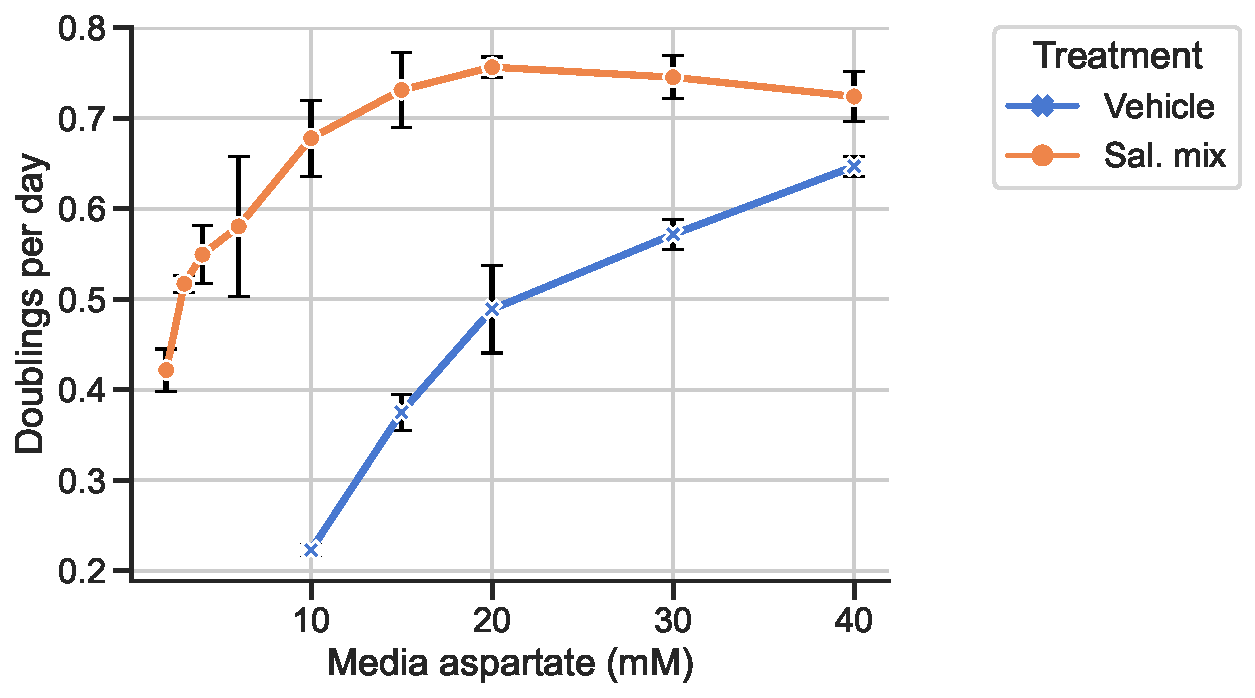
\includegraphics[width=0.65\textwidth]{figures/sapp/tRNA/H1299_GOT-DKO_prlfr.pdf}
    \caption[Asp titration in H1299 GOT DKO]{
    Proliferation assay with H1299 GOT DKO cells.
    Conditions with salvage mix (SM) contain: 500 µM asparagine, 200 µM uridine and 100 µM adenine.
    }
    \label{fig:sapp:ISR:H1299_DKO_prlfr}
\end{figure}


\begin{figure}[ht]
    \centering
    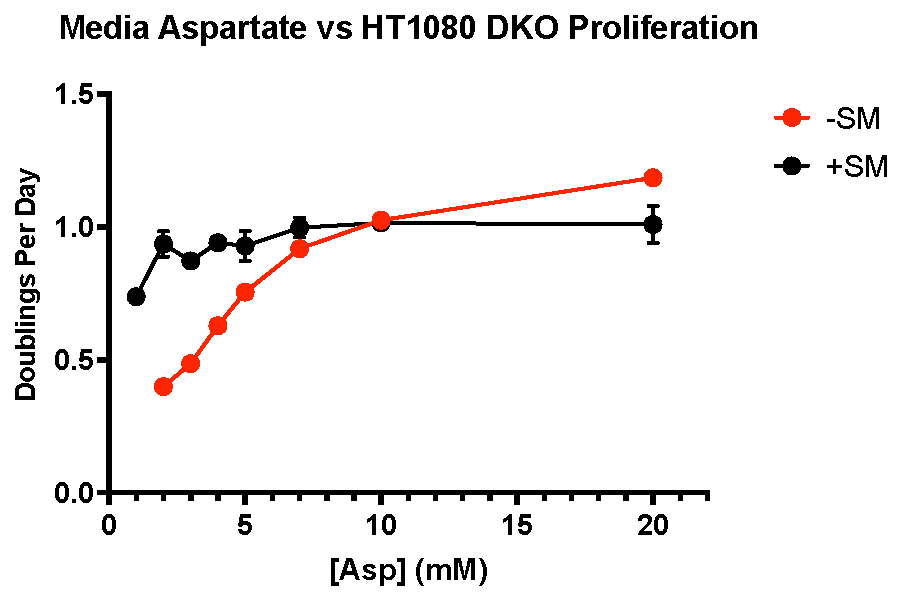
\includegraphics[width=0.65\textwidth]{figures/sapp/tRNA/HT1080_GOT-DKO_prlfr.pdf}
    \caption[Asp titration in H1080 GOT DKO]{
    Proliferation assay with HT1080 GOT DKO cells.
    Conditions with salvage mix (SM) contain: 500 µM asparagine, 200 µM uridine and 100 µM adenine.
    Made by David Sokolov.
    }
    \label{fig:sapp:ISR:HT1080_DKO_prlfr}
\end{figure}



\begin{figure}[ht]
    \centering
    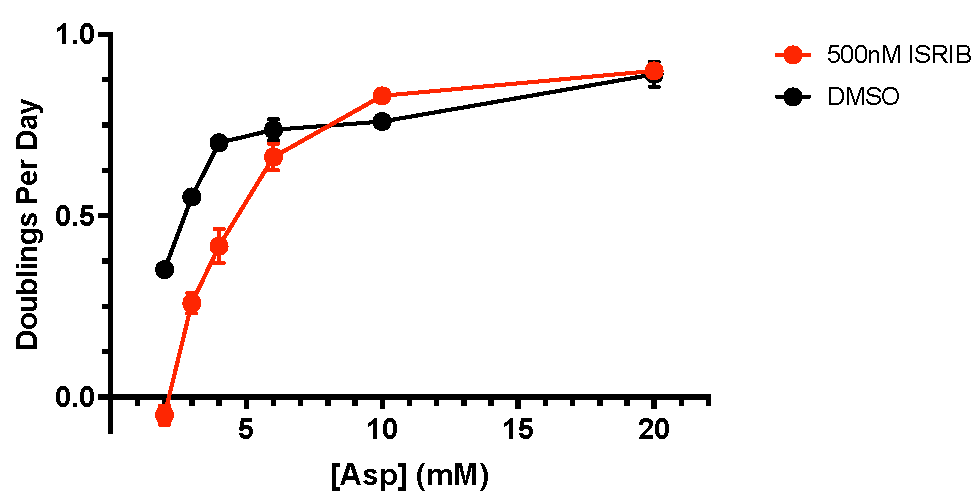
\includegraphics[width=0.65\textwidth]{figures/sapp/ISR/ISRIB-Exp2.pdf}
    \caption[Effect of ISR inhibition on HT1080 GOT DKO]{
    Proliferation assay with HT1080 GOT DKO cells and ISRIB as an inhibitor of ISR.
    Made by David Sokolov.
    }
    \label{fig:sapp:ISR:HT1080_DKO_ISRIB}
\end{figure}





\FloatBarrier
\section{Metabolic changes post aspartate depletion in GOT DKO}
To get insights into what else is going on during aspartate depletion in GOT DKO metabolites were extracted post aspartate depletion for 143B (figure \ref{fig:sapp:GOT_DKO_Asp_depl:143B_DKO_metab}) and HT1080 (figure \ref{fig:sapp:GOT_DKO_Asp_depl:HT1080_DKO_metab}).
Some metabolic changes are readily explained: intracellular aspartate decrease drastically and rapidly.
This is also the case for asparagine in 143B cells but in HT1080 cells asparagine only decreases 50 percent.
Fumarate and malate are decreased, probably due to lower asp consumption in purine synthesis and thus lower fumarate production.
Similarly, the IMP to AMP ratio is increased in both cell lines, probably due to low aspartate preventing IMP to AMP synthesis.
For 143B the pyrimidines metabolites decrease as expected during aspartate shortage; however, strangely pyrimidines metabolites increase in HT1080.
Similarly, differential effect is seen for succinate and glycerol 3-phosphate.

\begin{figure}[!ht]
     \centering
     \begin{subfigure}[b]{0.45\textwidth}
         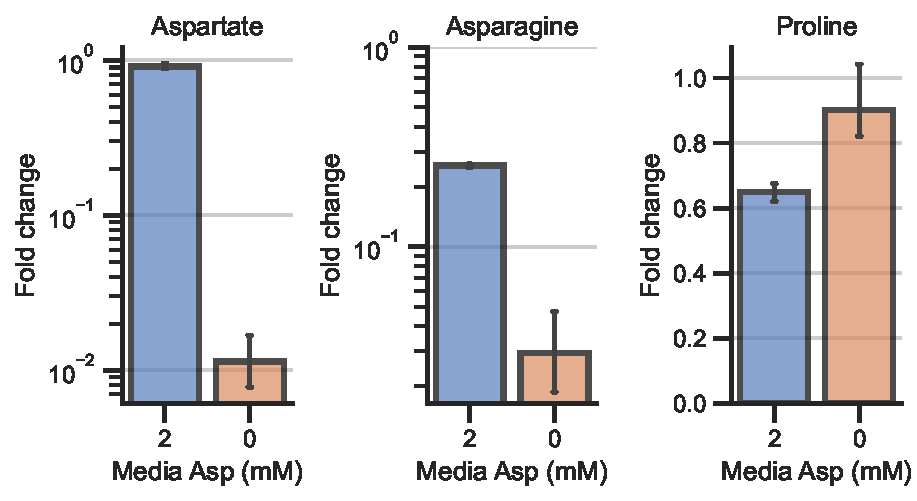
\includegraphics[width=\textwidth]{figures/sapp/GOT_DKO_Asp_depl/143B_DKO_AA.pdf}
         \caption{Amino acids}
         \label{fig:sapp:GOT_DKO_Asp_depl:143B_DKO_AA}
     \end{subfigure}
     \hspace{0.1\textwidth}
     \begin{subfigure}[b]{0.3\textwidth}
         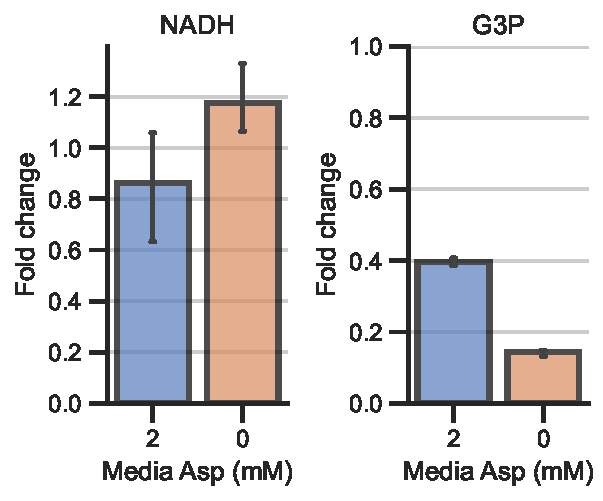
\includegraphics[width=\textwidth]{figures/sapp/GOT_DKO_Asp_depl/143B_DKO_rd.pdf}
         \caption{Redox metabolites}
         \label{fig:sapp:GOT_DKO_Asp_depl:143B_DKO_rd}
     \end{subfigure}
     \hfill
     \begin{subfigure}[b]{0.6\textwidth}
         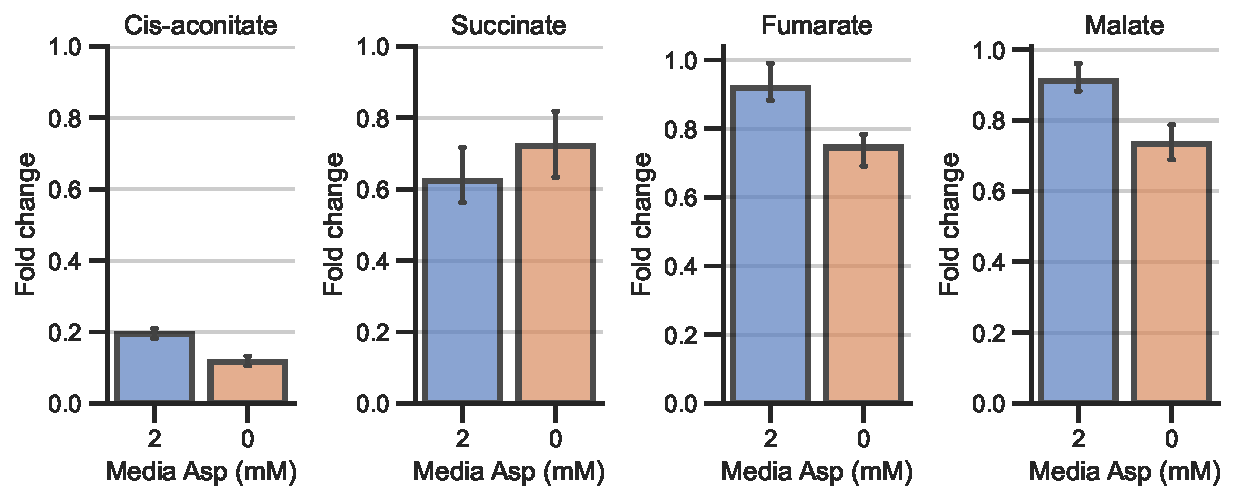
\includegraphics[width=\textwidth]{figures/sapp/GOT_DKO_Asp_depl/143B_DKO_tca.pdf}
         \caption{TCA metabolites}
         \label{fig:sapp:GOT_DKO_Asp_depl:143B_DKO_tca}
     \end{subfigure}
     \hfill
     \begin{subfigure}[b]{0.6\textwidth}
         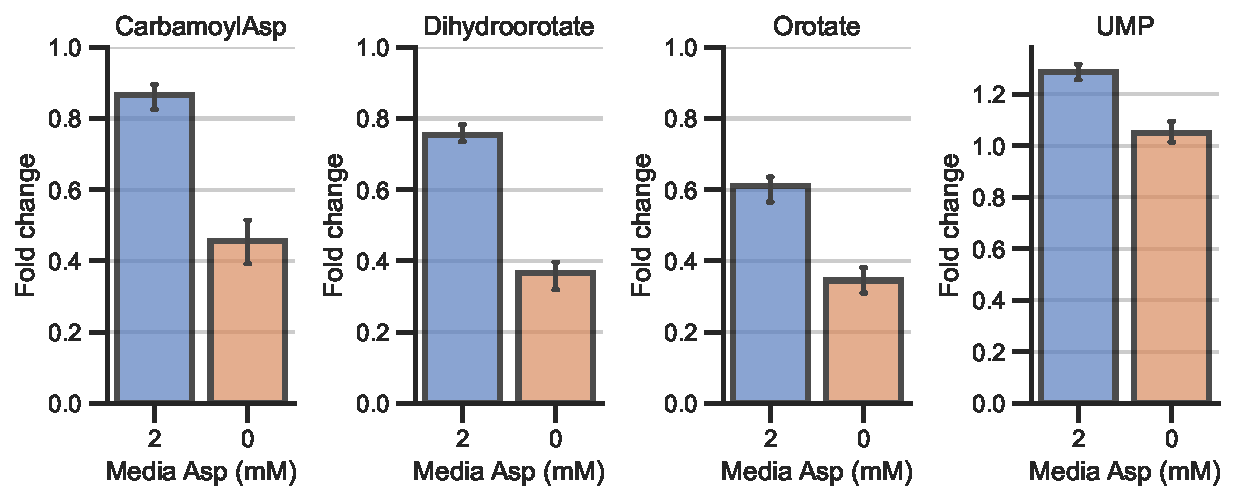
\includegraphics[width=\textwidth]{figures/sapp/GOT_DKO_Asp_depl/143B_DKO_pyr.pdf}
         \caption{Pyrimidine metabolites}
         \label{fig:sapp:GOT_DKO_Asp_depl:143B_DKO_pyr}
     \end{subfigure}
     \hfill
     \begin{subfigure}[b]{0.3\textwidth}
         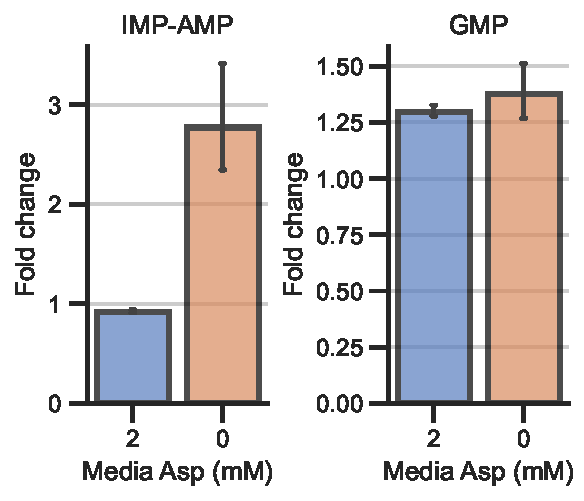
\includegraphics[width=\textwidth]{figures/sapp/GOT_DKO_Asp_depl/143B_DKO_pur.pdf}
         \caption{Purine metabolites}
         \label{fig:sapp:GOT_DKO_Asp_depl:143B_DKO_pur}
     \end{subfigure}
     \hfill
        \caption[Metabolic changes in 143B after Asp depl.]{
        Metabolic changes in 143B GOT DKO after aspartate depletion.
        Fold change compared to time zero 2 hours after media switch with/without aspartate.
        }
        \label{fig:sapp:GOT_DKO_Asp_depl:143B_DKO_metab}
\end{figure}


\begin{figure}[!ht]
     \centering
     \begin{subfigure}[b]{0.68\textwidth}
         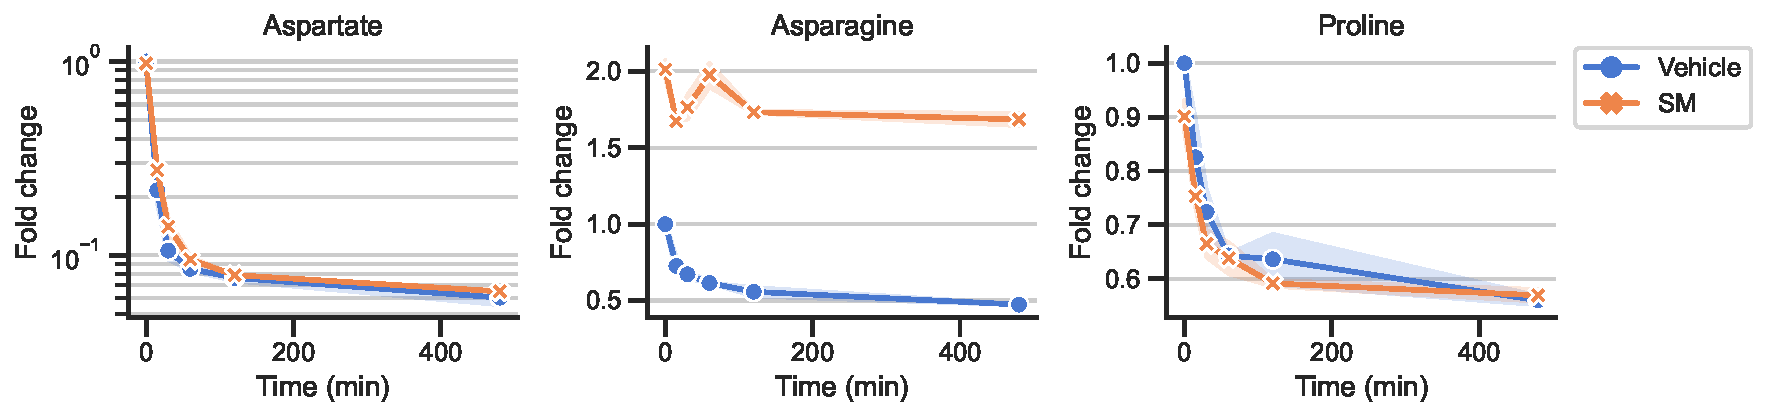
\includegraphics[width=\textwidth]{figures/sapp/GOT_DKO_Asp_depl/HT1080_DKO_AA.pdf}
         \caption{Amino acids}
         \label{fig:sapp:GOT_DKO_Asp_depl:HT1080_DKO_AA}
     \end{subfigure}
     \hfill
     \begin{subfigure}[b]{0.45\textwidth}
         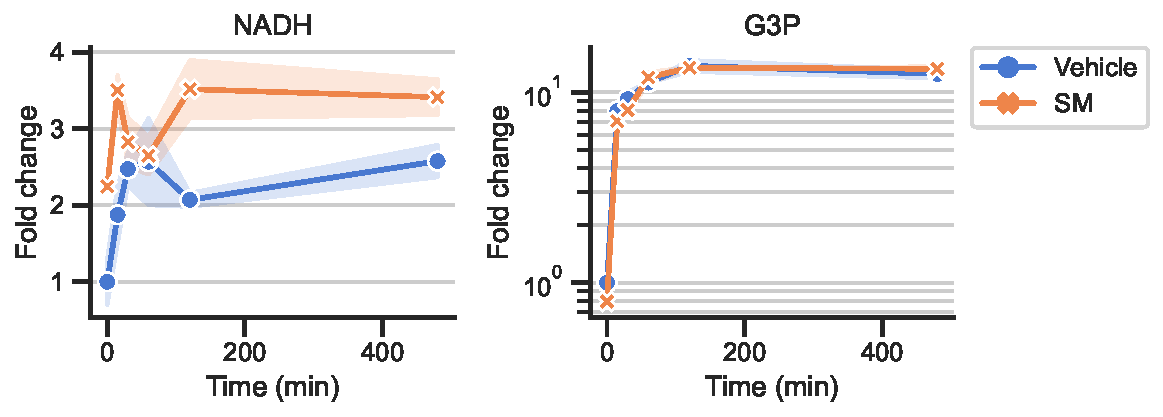
\includegraphics[width=\textwidth]{figures/sapp/GOT_DKO_Asp_depl/HT1080_DKO_rd.pdf}
         \caption{Redox metabolites}
         \label{fig:sapp:GOT_DKO_Asp_depl:HT1080_DKO_rd}
     \end{subfigure}
     \hfill
     \begin{subfigure}[b]{0.9\textwidth}
         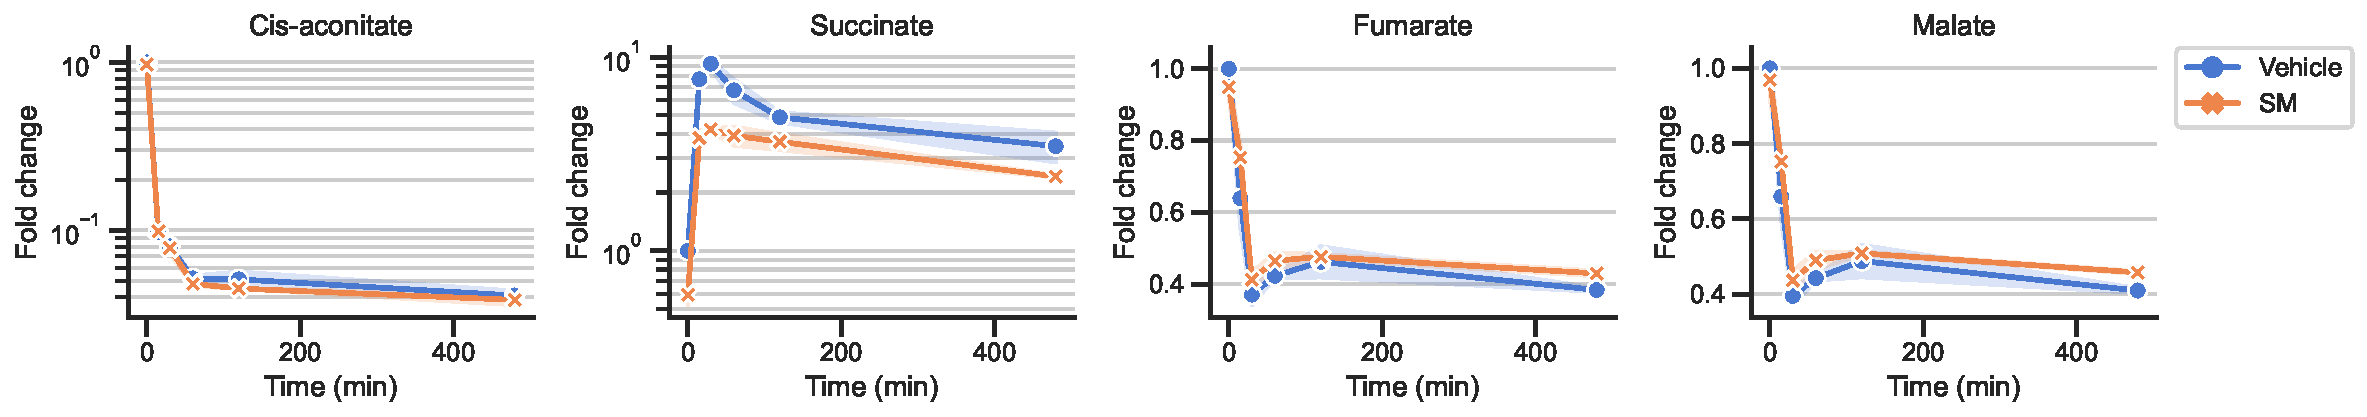
\includegraphics[width=\textwidth]{figures/sapp/GOT_DKO_Asp_depl/HT1080_DKO_tca.pdf}
         \caption{TCA metabolites}
         \label{fig:sapp:GOT_DKO_Asp_depl:HT1080_DKO_tca}
     \end{subfigure}
     \hfill
     \begin{subfigure}[b]{0.9\textwidth}
         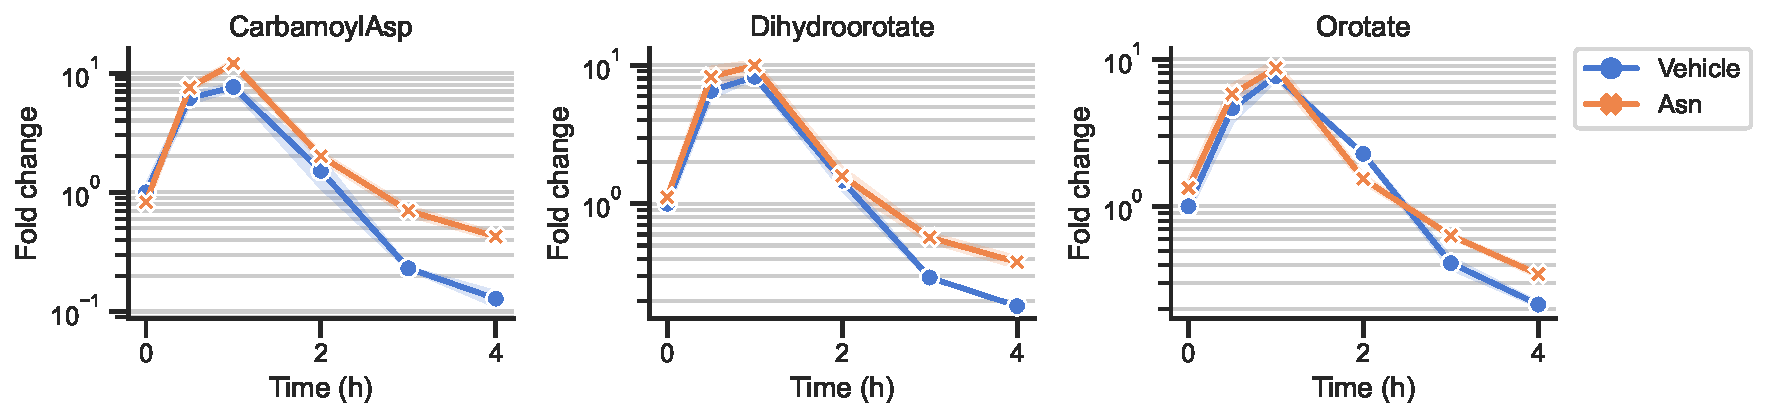
\includegraphics[width=\textwidth]{figures/sapp/GOT_DKO_Asp_depl/HT1080_DKO_pyr.pdf}
         \caption{Pyrimidine metabolites}
         \label{fig:sapp:GOT_DKO_Asp_depl:HT1080_DKO_pyr}
     \end{subfigure}
     \hfill
     \begin{subfigure}[b]{0.68\textwidth}
         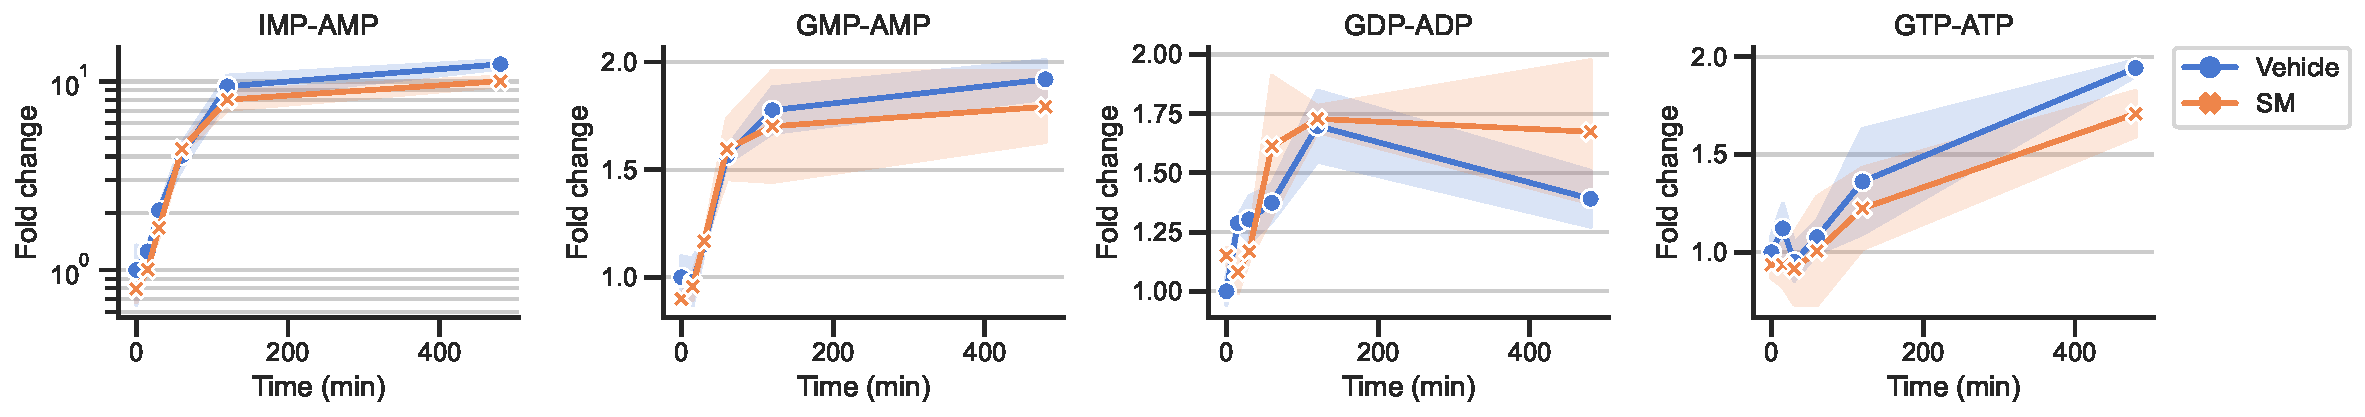
\includegraphics[width=\textwidth]{figures/sapp/GOT_DKO_Asp_depl/HT1080_DKO_pur.pdf}
         \caption{Purine metabolites (and dTTP)}
         \label{fig:sapp:GOT_DKO_Asp_depl:HT1080_DKO_pur}
     \end{subfigure}
     \hfill
        \caption[Metabolic changes in HT1080 after Asp depl.]{
        Metabolic changes in HT1080 GOT DKO after aspartate depletion.
        Time-series of fold changes, normalized to vehicle at time zero.
        Condition with salvage mix (SM) contains: 1 mM Asn/Urd, 0.5 mM Hpx, 20 µM adenine and 10 µM adenosine.
        }
        \label{fig:sapp:GOT_DKO_Asp_depl:HT1080_DKO_metab}
\end{figure}





\FloatBarrier
\section{Conclusions regarding ISR}
General observation regarding the ISR experiments:
\begin{itemize}
    \item Using multiple cell lines (143B, HT1080, H1299, 293T) appear to confuse the conclusion, but it also reveals that ISR activation has a cell line dependent component.
    An example of this would be the difference between 143B and H1299 in their tRNA charge response after ETC inhibitor treatment (figure \ref{fig:sapp:tRNA:143B_ETCinhib} and \ref{fig:sapp:tRNA:H1299_ETCinhib}).
    \item The GCN2iB inhibitor is likely having an off-target effect on HRI which affects the conclusion from Mick et al. \cite{Mick2020-kf} and a few of our own western blots.
    Using lower a concentration may mitigate this, although care must be taken not to use a concentration so low that it causes an unintended GCN2 activation as described by Carlson et al. \cite{Carlson2023-zh}.
    \item Aspartate limitation induced by mitochondrial inhibitors in WT cell is difficult to compare to aspartate limitation in GOT DKO cells.
    This is particularly evident when looking at tRNA charge, but it has also been observed on western blots were asparagine rescues ETC inhibitor induced ISR in WT cell but not aspartate depletion induced ISR in GOT DKO cells.
    \item ETC inhibitor induced ISR is very sensitive to media conditions e.g. media change will increase the asparagine depletion by efflux.
    Media change can also by itself cause ATF4 induction which is reversible with media asparagine (figure \ref{fig:app_ch2:sal_frac_conc}).    
    \item Time scale is an important factor to consider in a model over the observations e.g. mito-tRNA\textsuperscript{Asn} becomes uncharged before cyto-tRNA\textsuperscript{Asn} in 143B cells treated with antimycin (figure \ref{fig:sapp:tRNA:143B_Anti_time}).
    \item Proline is also a redox active amino acid and mito-tRNA\textsuperscript{Pro} charge is severely affected by some ETC inhibitors.
    This is concordant with very low mitochondrial proline concentrations, $\sim$10 µM reported by Chen et al. \cite{Chen2016-mf}.
    \item Asparagine supplementation, in the form of salvage mix, rescues mito-tRNA\textsuperscript{Asp} charge to a different extend in different cell lines e.g. compared 143B and HT1080 in figure \ref{fig:sapp:tRNA:DKO_Asp-Asn}.
    Besides offsetting aspartate consumption, asparagine could be deaminated by glutaminase, possibly explaining the difference in charge rescue.
\end{itemize}



\subsection{Proposed model}
For WT cells treatment with ETC inhibitors results in a complex tRNA charge response that is cell line and drug dependent but typically leads to uncharged mito-tRNA\textsuperscript{Asp}, mito-tRNA\textsuperscript{Asn} and/or mito-tRNA\textsuperscript{Pro}.
For 143B and HT1080 cells the induction of ISR can be ablated with asparagine and OMA1/HRI knockout and while asparagine only partially ablates ISR in 293T cells, knockout of GCN2 is also insufficient.
Meanwhile, mito-tRNA\textsuperscript{Asn} becomes substantially uncharged after just 30 minutes while cyto-tRNA\textsuperscript{Asn} maintains full charge for 7 hours.
Therefore, I hypothesize the following:
Treatment with ETC inhibitors induces ISR through uncharged mitochondrial tRNAs of either mito-tRNA\textsuperscript{Asp}, mito-tRNA\textsuperscript{Asn} and/or mito-tRNA\textsuperscript{Pro}.
The resulting eIF2alpha phosphorylation causes a global decrease in protein synthesis and for some cell line/drug combination this fully prevents accumulation of uncharged cytoplasmic tRNAs (H1299) whereas for other cell line/drug combinations this only delays the aspartate/asparagine depletion, sparing cyto-tRNA\textsuperscript{Asp}, cyto-tRNA\textsuperscript{Asn} charge for some time before eventual depletion and a secondary GCN2 mediated ISR.
This leads to a testable predictions regarding cell line specific observations and the timing of ISR vs. uncharged tRNA.
For example OMA1/HRI knockout ablates ETC inhibitor induced ISR in HT1080, and thus these cells should harbour no uncharged cytoplasmic tRNA, while on the other hand since we know that 143B WT cell do eventually accumulate uncharged cytoplasmic tRNA they should have a GCN2 mediated ISR even with OMA1/HRI knockout.
Another testable prediction would be related to proline and its effect on ISR which could be tested by proline supplementation.

For all GOT DKO cell lines mito-tRNA\textsuperscript{Asp} charge decreases as a function of aspartate; however, we know from DARS2 KO and rho0 cells of multiple cell lines that neither mito-tRNA\textsuperscript{Asp} charge nor indeed any mitochondrial tRNAs are necessary for aspartate depletion induced ISR.
Therefore, I hypothesize the following:
Decreasing media aspartate to a level still compatible with cell proliferation induces ISR through uncharged mito-tRNA\textsuperscript{Asp}, the resulting eIF2alpha phosphorylation causes a global decrease in protein synthesis and therefore cyto-tRNA\textsuperscript{Asp} remains charged (figure \ref{fig:sapp:tRNA:DKO_Asp-Asn}).
Complete aspartate removal leads to the above but then shortly after cyto-tRNA\textsuperscript{Asp} becomes uncharged due to insufficient aspartate (supported by data in figure \ref{fig:sapp:ISR:HT1080_DKO_ASPtit_time}).
Similarly, this is what will happen in DARS2 KO and rho0 cells where the initial wave of ISR from uncharged mito-tRNA\textsuperscript{Asp} is blunted but the subsequent decrease in cyto-tRNA\textsuperscript{Asp} charge will lead to GCN2 mediated ISR.
Thus, the hypothesis would predict that blocking ISR, e.g. through ISRIB, or blocking uncharged mito-tRNA\textsuperscript{Asp} mediated ISR through rho0, would lead to cells with uncharged cyto-tRNA\textsuperscript{Asp} upon aspartate limitation.

How could uncharged mitochondrial tRNA cause ISR?
Maybe by mitochondrial proteotoxic stress.
In this hypothesis an acute increase of uncharged tRNAs would lead to stalling and fall off of mitochondrial ribosomes, unfinished and unfolded proteins would be released and this would be the basis of proteotoxic stress.
Indeed, I have observed upregulation of mitochondrial protease LONP1 which is thought to be involved in degrading unfolded or misfolded proteins.
More recently, Fessler et al. \cite{Fessler2022-ho} and Sekine et al. \cite{Sekine2023-qh} have implicated mitochondrial proteotoxic stress and LONP1 directly in the HRI mediated activation of the ISR.
They showed that over-expression induced mitochondrial proteotoxic stress induces ISR through DELE1 and that DELE1 is normally degraded by LONP1 in the matrix but upon iron depletion becomes stabilized on the outer membrane to activate HRI and subsequent ISR.








Way forward:

Use GOT DKO mito vs. rho0 cells to 
(figure \ref{fig:sapp:ISR:143B_DKO_ISR}, bottom panel)


More time points
Proline









\FloatBarrier
\section{GOT DKO characterization}


\begin{figure}[!ht]
     \centering
     \begin{subfigure}[b]{0.8\textwidth}
         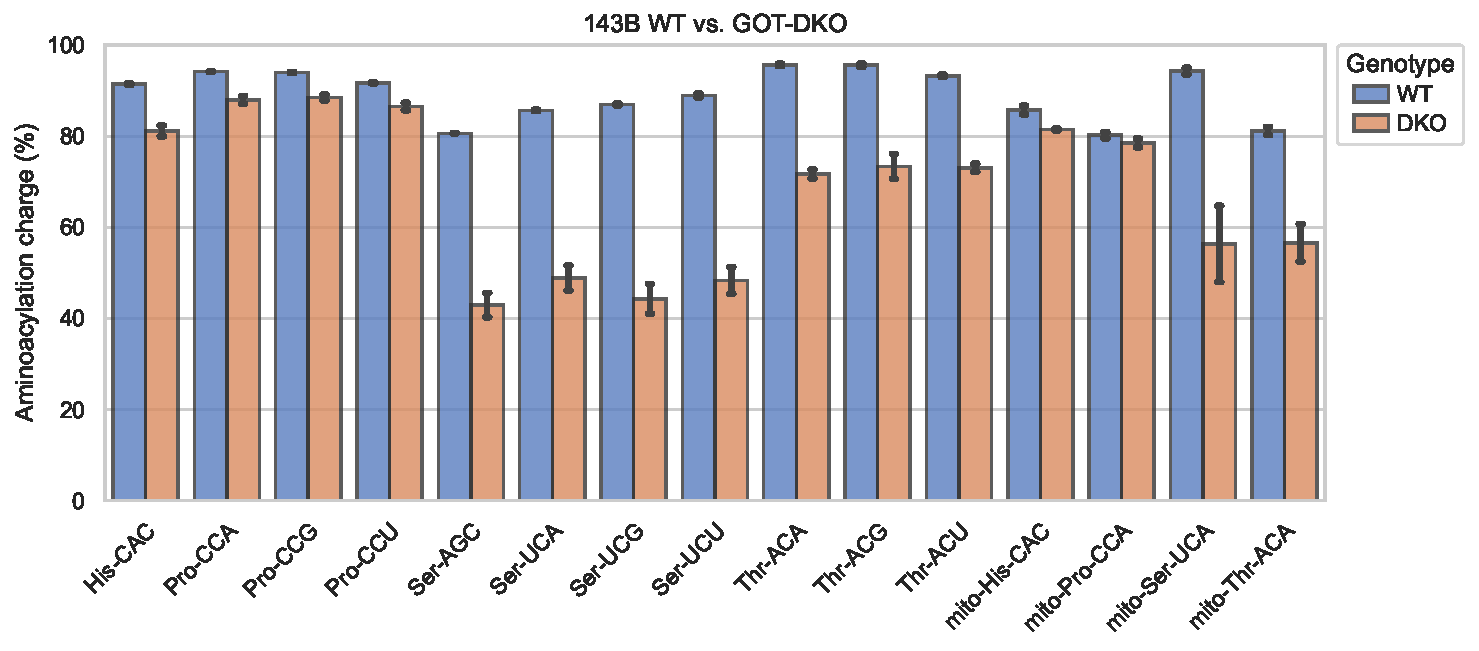
\includegraphics[width=\textwidth]{figures/sapp/DKO_char/143B-WT-DKO_charge.pdf}
     \end{subfigure}
     \begin{subfigure}[b]{0.8\textwidth}
         \vspace{2pt}
         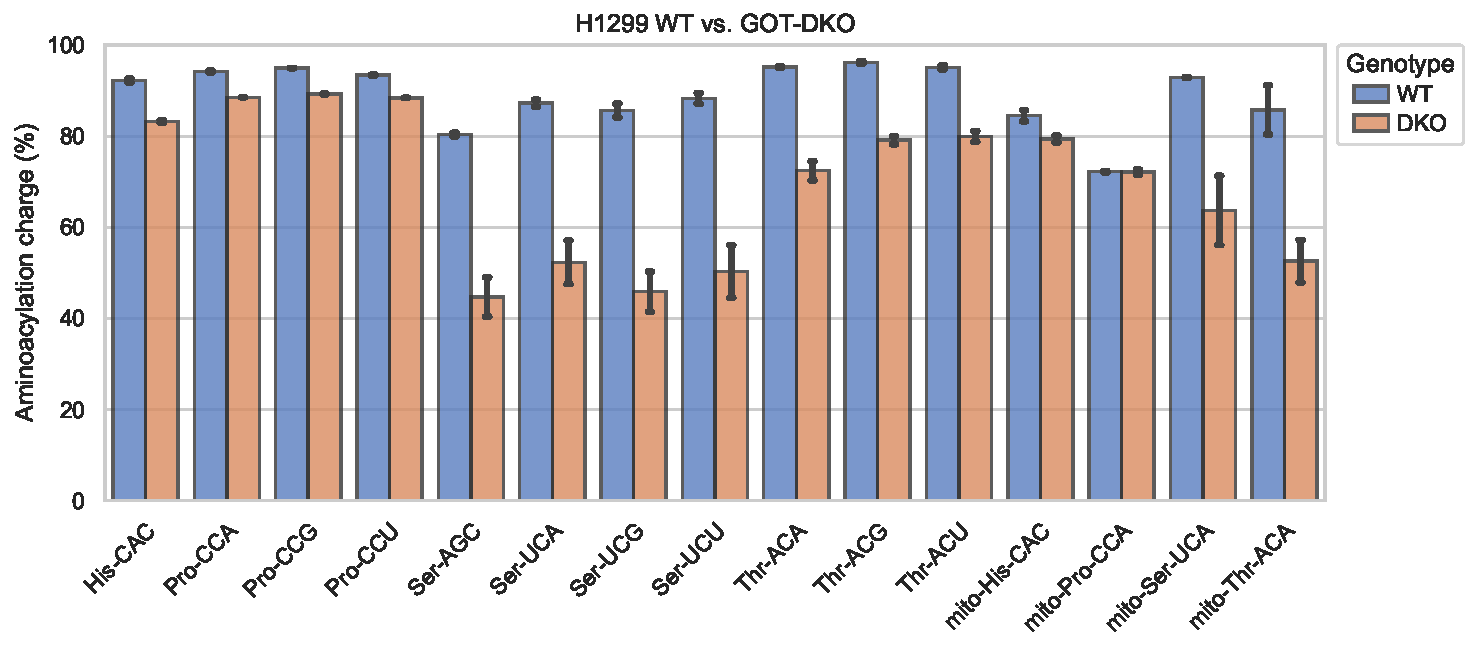
\includegraphics[width=\textwidth]{figures/sapp/DKO_char/H1299-WT-DKO_charge.pdf}
     \end{subfigure}
     \hfill
        \caption[tRNA charge in WT vs. GOT DKO]{
        tRNA charge in WT vs. DKO cell lines.
        For 143B GOT DKO, cells are in media with 20 mM Asp.
        For H1299 GOT DKO, cells are in media with 40 mM Asp.
        For other tRNAs (cytoplasmic as well as mitochondrial) GOT genotype had smaller or insignificant effect on charge.
        }
        \label{fig:sapp:tRNA:WT_vs_DKO}
\end{figure}


























